\documentclass[master=mcs]{kulemt}
\setup{
  title={Early-Stage Reconnaissance Detection in Operational Technology Networks Using Conntrack-Based Anomaly Detection},
  author={Maria Karegla},
  promotor={Prof.\,dr.\,ir.\ Bart Preneel \and Ir.\ Alex~Ongena},
  assessor={Ir.\,Kn. Owsmuch\and K. Nowsrest},
  assistant={Ir. Lode~Mertens \and Ir. Thibault Van Win}}
% Remove the "%" on the next line for generating the cover page
%\setup{coverpageonly}
% Remove the "%" before the next "\setup" to generate only the first pages
% (e.g., if you are a Word user).
%\setup{frontpagesonly}

% If you want to include other LaTeX packages, do it here. 

% Finally the hyperref package is used for pdf files.
% This can be commented out for printed versions.
\usepackage[pdfusetitle,colorlinks,plainpages=false]{hyperref}
\usepackage[table]{xcolor} % 'table'optie is handig voor cell backgrounds
\usepackage{xltabular}    % combinatie van longtable + tabularx
\usepackage[table]{xcolor}
\usepackage{enumitem}
\usepackage{xltabular,enumitem} 
\usepackage{xcolor}
\usepackage[table]{xcolor} 
\usepackage{tabularx}
\usepackage{pdflscape}
\usepackage{multirow}
\usepackage{tikz}
\usepackage{siunitx}
\usepackage{array}
\usepackage{makecell}
\usetikzlibrary{shapes.geometric, arrows.meta, positioning, calc}
\usepackage{graphicx}
\usepackage{booktabs}
\usepackage{xurl}
\usepackage{seqsplit}
\usepackage{subcaption}
\usepackage{adjustbox}
\usepackage{caption}
\usepackage{longtable}
\usepackage{seqsplit}
\newcommand{\feat}[1]{\texttt{\seqsplit{#1}}}
%%%%%%%
% The lipsum package is used to generate random text.
% You never need this in a real master's thesis text!
\IfFileExists{lipsum.sty}%
 {\usepackage{lipsum}\SetLipsumDefault{11-13}}%
 {\newcommand{\lipsum}[1][11-13]{\par And some text: lipsum ##1.\par}}
%%%%%%%
\usepackage{longtable}
%%%%%%%
%\includeonly{chapter-n}
\begin{document}

\begin{preface}
This is my acknowledgment to thank everyone who has kept me busy.
I would like to thank my supervisor, my advisor, and the entire jury.
My family has also been very supportive, of course.
\end{preface}

\tableofcontents*

\begin{abstract}
  This \texttt{abstract} environment provides a summary of the work, which may or may not be extensive.
The intention is that this should be limited to 1 page.

  \lipsum[1]
\end{abstract}

% A list of figures and tables is optional
%\listoffigures
%\listoftables
% If there are only a few figures and tables, it is better to use the following:
\listoffiguresandtables
% The list of symbols is also optional.
% This list must be created manually, e.g. as follows:
\chapter{List of abbreviations and symbols}
\section*{abbreviations}
\begin{flushleft}
  \renewcommand{\arraystretch}{1.1}
  \begin{tabularx}{\textwidth}{@{}p{12mm}X@{}}
    LoG   & Laplacian-of-Gaussian \\
    MSE   & Mean Square error \\
    PSNR  & Peak Signal-to-Noise ratio \\
  \end{tabularx}
\end{flushleft}
\section*{Symbols}
\begin{flushleft}
  \renewcommand{\arraystretch}{1.1}
  \begin{tabularx}{\textwidth}{@{}p{12mm}X@{}}
    42    & ``The Answer to the Ultimate Question of Life, the Universe,
            and Everything'' volgens de \cite{h2g2} \\
    $c$   & Speed of light \\
    $E$   & Energy \\
    $m$   & Mass \\
    $\pi$ & The number pi \\
  \end{tabularx}
\end{flushleft}

% Now comes the main text
\mainmatter

\chapter{Introduction}
\label{ch:introduction}
% on top of everything, the difficulty of compareing models in literature makes it hard to know what is really useful for my application
% talk about the pipeline starting from conntrack data
Modern industrial environments are becoming increasingly connected. Systems that were once largely isolated now communicate with enterprise networks, remote services, cloud platforms and security appliances~\cite{jeffrey_hybrid_2024}. This integration improves visibility, automation and operational efficiency, but it also increases the exposure of Operational Technology (OT) environments to cyber threats~\cite{behdadnia_early-stage_2025}. Unlike traditional Information Technology (IT) systems, attacks against OT environments may have consequences beyond data loss, including disruption of physical processes, equipment damage and safety risks~\cite{wang_guardians_2026, jeffrey_hybrid_2024}.

These characteristics make security monitoring in OT environments both important and challenging. Industrial networks often contain legacy devices, strict availability requirements and communication patterns that differ strongly between sites~\cite{abshari_survey_2025, jeffrey_hybrid_2024}. As a result, security mechanisms that are common in IT environments cannot always be transferred directly to OT environments~\cite{wang_guardians_2026}. Passive network-based monitoring is therefore an attractive approach, because it can observe communication behavior without modifying the industrial devices themselves~\cite{ortega-fernandez_network_2024}.

Anomaly detection is a promising technique in this context, since it can learn a reference of normal behavior and identify deviations from that reference. This is especially relevant when labeled attack data is limited or when the kind of attacks are unknown beforehand~\cite{jeffrey_hybrid_2024, meira_performance_2020}. However, the practical value of anomaly detection depends strongly on the data source, the feature representation, the thresholding strategy and the evaluation setting~\cite{fung_perspectives_2022}. Models that perform well on clean or controlled datasets may behave differently when applied to noisy operational data from real environments~\cite{catillo_cps-guard_2023, moriano_adaptive_2025}.

This thesis was carried out in collaboration with ''AXS Guard (by Appraoch Cyber)'', whose security appliances are deployed at the network edge of customer environments. Because these appliances already operate as routers and firewalls, they naturally observe the connections passing through them. This makes Linux connection tracking metadata, or conntrack metadata, a practical data source for anomaly detection, as it provides lightweight summaries of observed network connections without requiring changes to OT devices or relying on deep packet inspection, which can introduce additional processing overhead, privacy concerns and deployment complexity, especially when traffic is encrypted or difficult to parse reliably. The choice for conntrack metadata is therefore motivated not only by its technical content, but also by its deployability in real customer environments.

In this thesis, this metadata is transformed into window-based feature vectors and used to evaluate whether existing unsupervised anomaly detection models can detect early-stage reconnaissance behavior. Reconnaissance is considered because it often precedes more intrusive attack phases, such as exploitation or lateral movement~\cite{behdadnia_early-stage_2025}. During this phase, an attacker attempts to discover active hosts, reachable services and communication paths in order to identify possible entry points or targets. Detecting these activities early can give defenders time to investigate or respond before the attacker progresses toward actions that may disrupt the physical process. Since reconnaissance mainly affects communication patterns, it can leave traces in network metadata even before the physical process itself is affected~\cite{zaidy_comprehensive_2025, cabana_detecting_2019}.



The goal of this thesis is not to design a new anomaly detection algorithm, but to implement and evaluate existing unsupervised models as part of a consistent detection pipeline. The pipeline covers the transformation of raw conntrack events into flow records, the aggregation of these records into time windows, the extraction and selection of features, model training on benign data, threshold selection and evaluation on operational data with simulated reconnaissance attacks.

The central research question of this thesis is formulated as follows:



\begin{center}
\setlength{\fboxsep}{8pt}
\fbox{%
\begin{minipage}{0.9\textwidth}
% \centering
\textit{How can existing unsupervised anomaly detection models be adapted, implemented as a pipeline, and evaluated using Linux connection tracking metadata to detect early-stage reconnaissance in noisy, real-world OT environments?}
\end{minipage}
}
\end{center}



To answer this question, a pipeline is constructed where the following steps are carried out:

\begin{itemize}
    \item reconstruct raw Linux conntrack events into connection-level records that can be used for network traffic analysis

    \item aggregate the reconstructed connections into time-based windows per source host, so that each window can be represented as a feature vector

    \item define and select conntrack-derived features that capture behaviours relevant to reconnaissance, such as destination spread, short-lived communication and asymmetric or failed connections

    \item simulate early-stage reconnaissance scenarios and inject them into noisy operational OT traffic to create an evaluation setting

    \item apply and configure existing unsupervised anomaly detection models, including k-NN, K-Means and autoencoder-based approaches, to the extracted conntrack-based feature vectors

    \item compare the models under a consistent experimental pipeline, considering the effect of design choices such as window length, feature set, threshold selection and evaluation metric.
\end{itemize}


The remainder of this thesis is structured as follows. Chapter~\ref{ch:related_work} discusses related work on OT security, anomaly detection, reconnaissance, unsupervised models and evaluation metrics. Chapter~\ref{ch:dataset} describes the data source, preprocessing steps and construction of the experimental datasets. Chapter~\ref{ch:detection_methodology} presents the detection pipeline and experimental setup. Chapter~\ref{ch:results} reports and discusses the results. Finally, Chapter~\ref{ch:conclusion} summarizes the main findings and future work.

% This main question is divided into the following subquestions:

% \begin{itemize}
%     \item What information can be extracted from Linux connection tracking metadata, and how can it be represented in a form suitable for anomaly detection?

%     \item Why is noisy operational OT data an important evaluation setting for anomaly detection models?

%     \item Why is early-stage reconnaissance a relevant target for OT anomaly detection, and how can it be reflected in network metadata?

%     \item How do existing unsupervised anomaly detection models, such as k-NN, K-Means and autoencoder-based approaches, perform when adapted to conntrack-derived OT features?

%     \item How can these models be compared under a consistent pipeline, and how do design choices such as feature selection, window length, thresholding and evaluation metrics affect the interpretation of their performance?
% \end{itemize}





\chapter{Related Work}
\label{ch:related_work}
\section{Operational Technology Networks and Security Challenges}
\label{sec:ot_security_challenges}
Operational Technology (OT) refers to the hardware and software systems utilized for the direct monitoring, control, and actuation of physical devices, industrial processes, and events~\cite{kapoor_cyber_2025} They include components such as sensors, actuators, Programmable Logic Controllers (PLCs), Remote Terminal Units (RTUs), Supervisory Control and Data Acquisition (SCADA) systems, Human-Machine Interfaces (HMIs), and engineering workstations.  These systems form the basis of many Cyber-Physical Systems (CPS) and are used in critical infrastructure such as power grids, water treatment facilities, transportation networks and manufacturing plants~\cite{wang_guardians_2026}.

Historically, OT networks operated as isolated, air-gapped environments that relied almost entirely on physical separation for security~\cite{jeffrey_hybrid_2024}. This separation has changed with the adoption of Industry 4.0, an industrial paradigm that describes the digital transformation of manufacturing and other industrial sectors through connected, automated and data-driven systems. The Industrial Internet of Things (IIoT) is part of this shift and involves the connection of  industrial sensors, devices and machines to networks for data exchange, remote monitoring and automation. As a result, OT environments are increasingly integrated with traditional IT networks. While this IT-OT convergence improves data collection, automation and operational efficiency, it also expands the cyber-attack surface. Industrial assets that were once assumed to be isolated may become reachable from corporate networks, external services, or indirectly through compromised IT systems~\cite{kapoor_cyber_2025, jeffrey_hybrid_2024}.

Securing these environments is difficult because IT and OT networks do not always have the same operational priorities.  In traditional IT security, these priorities are often described using the CIA triad: Confidentiality, Integrity and Availability. Confidentiality protects information from unauthorized access, Integrity protects data and systems from unauthorized modification, and Availability ensures that systems remain accessible when needed. In traditional IT environmens, confidentiality often has the highest priority, followed by integraity and lastly availability. In OT environments, however, this ordering is reversed towards an AIC perspective, with availability being the main concern. This is because OT systems are directly connected to physical processes and are often subject to real-time and safety constraints. Downtime, delayed communication, or incorrect control actions can lead not only to data loss or service disruption, but also to production loss, equipment damage, environmental impact or risks to human safety~\cite{abshari_survey_2025, kapoor_cyber_2025}.



These risks have already been demonstrated by several well-known cyber-physical attacks. Stuxnet targeted Siemens PLCs used in an Iranian nuclear facility and is often considered one of the first examples of malware causing direct physical damage in an industrial process. It modified the control logic of uranium-enrichment centrifuges so that they operated outside safe conditions, while simultaneously hiding this abnormal behavior from monitoring systems by reporting normal-looking values~\cite{kapoor_cyber_2025, cabana_detecting_2019}. BlackEnergy and Industroyer later showed how attacks against power-grid environments can move beyond compromise of IT systems and directly affect electricity distribution. In the Ukrainian power-grid incidents, attackers interacted with industrial control systems and protocols to disrupt substations and cause real power outages~\cite{kapoor_cyber_2025, cabana_detecting_2019}. Triton/Trisis targeted Schneider Electric Triconex Safety Instrumented Systems in a petrochemical plant. This was especially concerning because safety instrumented systems are designed to keep industrial processes within safe operating limits, meaning that the attack targeted not only production systems but also the mechanisms intended to prevent catastrophic failures~\cite{kapoor_cyber_2025, wang_guardians_2026}. More recent ransomware incidents, such as EKANS and Colonial Pipeline, further show that cyber incidents do not need to directly manipulate PLC logic to affect industrial operations. EKANS included functionality to terminate industrial control processes, while the Colonial Pipeline incident led to a multi-day shutdown of fuel pipeline operations~\cite{kapoor_cyber_2025,  ding_data-driven_2022}. This illustrates why OT security has to consider cyber-physical consequences, not only traditional information security risks.

Furthermore, the deployment of security solutions in OT is often limited by legacy systems and resource constraints. Many OT environments still rely on older devices and industrial protocols, such as Modbus, DNP3 and EtherNet/IP, which were designed mainly for reliable communication and not necessarily with built-in security mechanisms such as encryption or strong authentication~\cite{wang_guardians_2026, kapoor_cyber_2025}. Updating or replacing such systems can be operationally risky, expensive, or delayed because of uptime requirements~\cite{abshari_survey_2025, kapoor_cyber_2025}. In addition, endpoint devices at the lower levels of an ICS architecture, such as sensors, actuators and PLCs, often have limited memory and computational resources~\cite{abshari_survey_2025, jeffrey_hybrid_2024}. This makes it difficult to deploy heavy host-based security mechanisms directly on these devices.


For these reasons, it is important to explore security approaches that are adapted to OT environments. Any monitoring or detection method has to take into account the operational constraints of industrial systems, where availability, safety and continuity are central requirements. At the same time, the method should be deployable without major changes to legacy devices or interruptions of the physical process. This is a difficult balance. OT environments need better visibility into suspicious behavior, but the security mechanism itself should not become a source of operational risk. The next section therefore discusses anomaly detection as a possible approach for detecting abnormal behavior in OT networks.


\section{Anomaly Detection in OT Environments}
Given the constraints discussed in Section~\ref{sec:ot_security_challenges}, OT security mechanisms should provide visibility into suspicious behavior without disrupting the underlying physical process. Intrusion Detection Systems (IDS) are one way to provide this visibility and are commonly divided into signature-based and anomaly-based approaches. Signature-based IDS compare observed traffic or system events against predefined rules or patterns, known as signatures, that describe previously identified malicious activity. This makes them effective for attacks that have already been characterized, but less suitable for novel or targeted attacks whose signatures are not yet availabl~\cite{meira_performance_2020, jeffrey_hybrid_2024} This limitation is especially relevant in OT environments, where attacks may be highly system-specific and where generating signatures for complex process or network behavior can be difficult~\cite{wang_guardians_2026}.

Anomaly-based detection takes a different approach: instead of searching for known attack patterns, normal behavior is modeled based on observed data, and deviations from this model are flagged as suspicious~\cite{abshari_survey_2025}. Anomaly detection has been studied extensively in IT security, but methods developed for general IT traffic cannot simply be assumed to transfer directly to OT environments. IT traffic is often shaped by human activity, web applications, cloud services and changing user behavior, making it diverse and highly variable. OT traffic, in contrast, is more closely tied to the physical process and is often driven by fixed interactions between devices, periodic control tasks, polling behavior and stable asset roles. This makes anomaly detection attractive for OT networks, where unknown attacks are an important concern and where communication is often more regular than in general IT networks. This periodic nature of OT networks, means deviations from expected communication can provide more useful indicators of abnormal behavior.~\cite{meira_performance_2020, catillo_cps-guard_2023}. 

However, this regularity does not mean that a single generic baseline can be applied to all OT networks. Jeffrey et al.~\cite{jeffrey_hybrid_2024} describe IT networks as being closer to a ``monoculture'', with many similar systems and more standardized communication protocols, while OT networks are much more heterogeneous and differ strongly between organizations. A pattern that is normal in one industrial environment may therefore be unusual in another. For this reason, OT anomaly detection cannot simply reuse IT-based methods or generic traffic models, but requires environment-specific baselines that capture the temporal and asset-level behavior of the monitored operational context~\cite{jeffrey_hybrid_2024}.



A major challenge in developing machine learning-based anomaly detection for OT environments is the limited availability of labeled attack data. Cyberattacks on critical infrastructure are rare, difficult to observe, and unsafe to reproduce in operational environments. As a result, real-world OT datasets are often dominated by benign traffic, while labeled malicious examples are scarce or unavailable~\cite{jeffrey_hybrid_2024, wang_guardians_2026}. This makes fully supervised learning difficult, since such models require representative examples of both normal and attack behavior. Even when attack labels are available in public datasets, they may not cover the full range of realistic attacks or environment-specific behavior. For this reason, one-class and semi-supervised approaches are frequently used in OT anomaly detection~\cite{catillo_cps-guard_2023, jeffrey_hybrid_2024, meira_performance_2020}. In this setting, the model is trained mainly or exclusively on benign data and learns a representation of normal operation. During detection, samples that deviate sufficiently from this learned normal behavior receive a high anomaly score.

\section{Limitations of Existing OT Anomaly Detection}

Although one-class and semi-supervised anomaly detection methods are a practical direction for OT networks, existing research still has several limitations that make it difficult to transfer results to real operational environments. A first limitation is the strong reliance on a small number of public benchmark datasets, such as SWaT, WADI and BATADAL~\cite{atluri_perspectives_2022, abshari_survey_2025}. These datasets are valuable because they provide labeled attack scenarios and allow different methods to be tested on a common baseline. However, they are usually collected in controlled test environments and therefore do not fully represent the conditions found in real OT networks. Operational environments can contain noisy traffic, benign misconfigurations, maintenance activity, incomplete labels or customer-specific behavior that are difficult to capture in benchmark datasets~\cite{moriano_adaptive_2025, jeffrey_hybrid_2024}. As a result, models that perform well on clean and controlled datasets may not generalize directly to real, noisy environments.

Another limitation is that results across OT anomaly detection studies are difficult to compare directly. Existing work evaluates a wide range of methods, from distance-based and clustering approaches to tree-based outlier detectors and deep reconstruction-based models, but these are often tested with different datasets, preprocessing steps, feature sets, thresholding strategies and model configurations~\cite{wang_guardians_2026, atluri_perspectives_2022}. As a result, it is difficult to determine whether a reported improvement is caused by the model architecture itself, by the data pipeline, or by the evaluation setup. If models cannot be compared under consistent conditions, it is also difficult to decide which approach is actually suitable for a specific OT monitoring problem. Recent evaluations further show that preprocessing choices and detection hyperparameters can strongly influence the final result, while the specific model architecture is not always the dominant factor~\cite{atluri_perspectives_2022}. Hence comparing candidate models within the same data pipeline and evaluation setup leads to more useful conclusions rather than treating reported performance numbers from different studies as directly comparable.

A final limitation of much OT anomaly detection research is that it focuses mainly on physical process variables, such as sensor readings, actuator states, tank levels or other process measurements. This is natural for datasets such as SWaT and WADI, where attacks are often represented through changes in the physical process. However, it also means that many proposed methods are evaluated on attacks that have already affected the process itself~\cite{atluri_perspectives_2022, behdadnia_early-stage_2025}. Less attention is given to earlier network-level activity, such as host discovery, port scanning or other reconnaissance behaviour, even though these actions may occur before direct manipulation of the physical infrastructure.



\section{Early-Stage Detection and Reconnaissance}
\label{sec:early_stage_detection}

The focus on physical process variables can be understood through the Cyber Kill Chain (CKC), which as depicted in Figure~\ref{fig:cyber_kill_chain}, describes an intrusion as a sequence of stages: reconnaissance, weaponization, delivery, exploitation, installation, command and control, and action on objectives~\cite{behdadnia_early-stage_2025}. In the early stages, the attacker gathers information about the target environment, prepares or delivers the attack, and attempts to gain a foothold. In the later stages, the attacker establishes persistence, communicates with compromised systems, and ultimately executes their objective. In an OT context, this final objective may involve manipulating the physical process, for example through false data or command injection~\cite{behdadnia_early-stage_2025}. Process-level anomaly detection mainly observes these later stages, where the attacker has already reached the point of affecting the physical infrastructure. While such detection is still important, it leaves less time for operators to react before operational consequences occur.

For this reason, early-stage detection has become an important direction for OT security. The initial stages of an intrusion can last much longer than the final execution phase, providing defenders with more time to detect suspicious behavior and respond before the attack reaches its objective~\cite{behdadnia_early-stage_2025}

Reconnaissance is especially relevant in this context because it is often one of the first steps performed by an attacker. Before exploiting a target, the attacker typically tries to understand the network by identifying active hosts, open ports, exposed services and possible entry points. This can involve host discovery, port scanning and service enumeration~\cite{keshavamurthy_early_2023, cabana_detecting_2019}. These activities cannot be observed through physical processes but leave observable traces in network communication, such as connections to many destinations, probes to many ports, short-lived TCP flows or failed connection attempts. Detecting such patterns can provide an early warning before the attacker moves further along the kill chain~\cite{zaidy_comprehensive_2025, ring_detection_2018}.



% \begin{figure}[htbp]
%     \centering
%     \makebox[\textwidth][c]{%
%     \begin{adjustbox}{width=1.3\textwidth}
%     \begin{tikzpicture}[
%         tactic/.style={
%             rectangle,
%             rounded corners=2pt,
%             draw=black!60,
%             minimum width=2.15cm,
%             minimum height=0.75cm,
%             align=center,
%             font=\footnotesize,
%             text width=1.75cm
%         },
%         normal/.style={tactic, fill=blue!10},
%         focus/.style={tactic, fill=green!18},
%         impact/.style={tactic, fill=red!18}
%     ]

%     \node[normal] (initial) {Initial\\Access};
%     \node[normal, right=0.20cm of initial] (execution) {Execution};
%     \node[normal, right=0.20cm of execution] (persistence) {Persistence};
%     \node[normal, right=0.20cm of persistence] (privilege) {Privilege\\Escalation};
%     \node[normal, right=0.20cm of privilege] (evasion) {Evasion};
%     \node[focus, right=0.20cm of evasion] (discovery) {Discovery};
%     \node[normal, right=0.20cm of discovery] (lateral) {Lateral\\Movement};
%     \node[normal, right=0.20cm of lateral] (collection) {Collection};
%     \node[normal, right=0.20cm of collection] (c2) {Command\\and Control};
%     \node[impact, right=0.20cm of c2] (inhibit) {Inhibit\\Response\\Function};
%     \node[impact, right=0.20cm of inhibit] (impair) {Impair\\Process\\Control};
%     \node[impact, right=0.20cm of impair] (impactnode) {Impact};

%     \node[above=0.18cm of discovery, font=\footnotesize\bfseries, text=green!45!black]
%         {Focus of this thesis};

%     \node[below=0.18cm of impair, font=\footnotesize\bfseries, text=red!60!black]
%         {Physical/process impact};

%     \end{tikzpicture}
%     \end{adjustbox}%
%     }
%     \caption{MITRE ATT\&CK for ICS tactics.}
%     \label{fig:mitre_attack_ics_tactics}
% \end{figure}

\begin{figure}[htbp]
    \centering
    \makebox[\textwidth][c]{%
    \begin{adjustbox}{width=1.3\textwidth}
    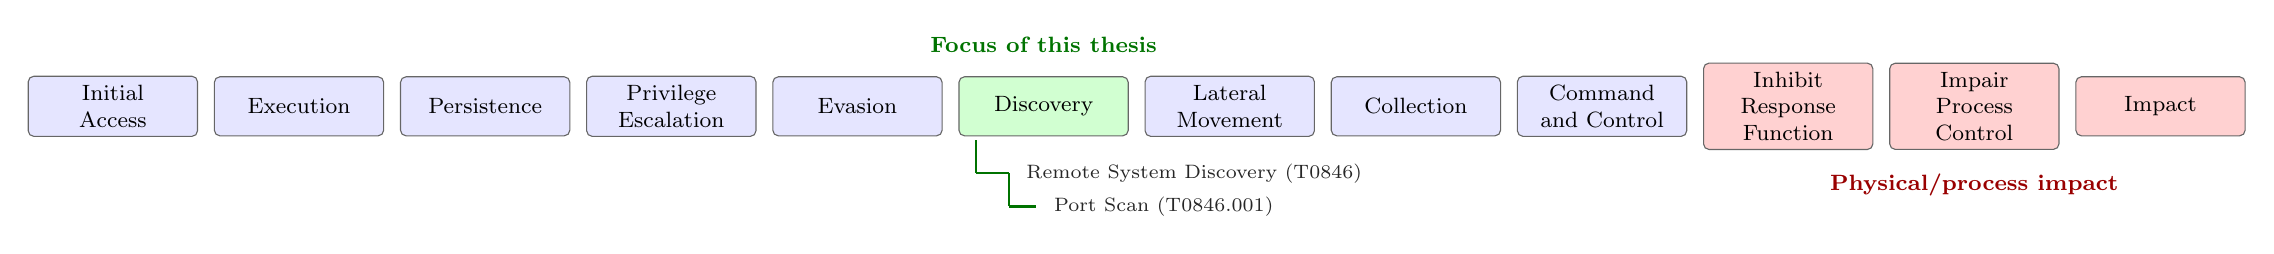
\begin{tikzpicture}[
        tactic/.style={
            rectangle,
            rounded corners=2pt,
            draw=black!60,
            minimum width=2.15cm,
            minimum height=0.75cm,
            align=center,
            font=\footnotesize,
            text width=1.75cm
        },
        normal/.style={tactic, fill=blue!10},
        focus/.style={tactic, fill=green!18},
        impact/.style={tactic, fill=red!18},
        techlabel/.style={
            anchor=west,
            font=\scriptsize,
            align=left,
            text=black!85
        }
    ]

    % Main tactic row
    \node[normal] (initial) {Initial\\Access};
    \node[normal, right=0.20cm of initial] (execution) {Execution};
    \node[normal, right=0.20cm of execution] (persistence) {Persistence};
    \node[normal, right=0.20cm of persistence] (privilege) {Privilege\\Escalation};
    \node[normal, right=0.20cm of privilege] (evasion) {Evasion};
    \node[focus, right=0.20cm of evasion] (discovery) {Discovery};
    \node[normal, right=0.20cm of discovery] (lateral) {Lateral\\Movement};
    \node[normal, right=0.20cm of lateral] (collection) {Collection};
    \node[normal, right=0.20cm of collection] (c2) {Command\\and Control};
    \node[impact, right=0.20cm of c2] (inhibit) {Inhibit\\Response\\Function};
    \node[impact, right=0.20cm of inhibit] (impair) {Impair\\Process\\Control};
    \node[impact, right=0.20cm of impair] (impactnode) {Impact};

    % Labels
    \node[above=0.18cm of discovery, font=\footnotesize\bfseries, text=green!45!black]
        {Focus of this thesis};

    \node[below=0.18cm of impair, font=\footnotesize\bfseries, text=red!60!black]
        {Physical/process impact};

    % ------------------------------------------------------------------
    % Discovery branch: moved toward the LEFT side of the Discovery box
    % ------------------------------------------------------------------

    % Start near left side of Discovery box, not in the center
    \coordinate (discstart) at ($(discovery.south west)+(0.22cm,-0.05cm)$);

    % First level: Remote System Discovery
    \coordinate (remotelevel) at ($(discstart)+(0,-0.42cm)$);
    \draw[thick, green!45!black] (discstart) -- (remotelevel);
    \draw[thick, green!45!black] (remotelevel) -- ++(0.42cm,0) coordinate (remoteend);
    \node[techlabel] at ($(remoteend)+(0.10cm,0)$)
        {Remote System Discovery (T0846)};

    % Second level: Port Scan as sub-technique of Remote System Discovery
    \coordinate (subvertend) at ($(remoteend)+(0,-0.42cm)$);
    \draw[thick, green!45!black] (remoteend) -- (subvertend);
    \draw[thick, green!45!black] (subvertend) -- ++(0.35cm,0) coordinate (portend);
    \node[techlabel] at ($(portend)+(0.10cm,0)$)
        {Port Scan (T0846.001)};

    \end{tikzpicture}
    \end{adjustbox}%
    }
    \caption{MITRE ATT\&CK for ICS tactics and the Discovery-related behaviour studied in this thesis.}
    \label{fig:mitre_attack_ics_tactics}
\end{figure}

\section{Unsupervised Models for Network-Based Anomaly Detection}
\label{sec:literature_models}
To detect the early-stage reconnaissance activities discussed in Section~\ref{sec:early_stage_detection}, multiple unsupervised and semi-unsupervised models were explored that can identify deviations in network traffic without relying on known attack signatures. 

Distance-based algorithms, and especially k-Nearest Neighbours (k-NN), are frequently used as lightweight anomaly detection models~\cite{meira_performance_2020, jeffrey_hybrid_2024, cai_adam_2023}. In a one-class setting, k-NN stores benign reference samples and scores a new observation according to its distance from the closest benign samples.  Meira et al.~\cite{meira_performance_2020} evaluated several unsupervised techniques for cyber-attack anomaly detection on the public NSL-KDD and ISCX network intrusion datasets, including One-Class Nearest Neighbour, One-Class K-Means, Isolation Forest, One-Class SVM and an autoencoder. Their results show that nearest-neighbour methods can perform competitively on network intrusion data, especially on the ISCX dataset~\cite{meira_performance_2020}. Jeffrey et al. also motivate the use of one-class models in CPS environments, arguing that malicious data is often scarce and that modelling benign behaviour directly is more suitable than relying on balanced two-class training data~\cite{jeffrey_hybrid_2024}. In their experiments, one-class k-NN achieved the best accuracy among the evaluated one-class and two-class models, which supports its use as a simple but strong baseline~\cite{jeffrey_hybrid_2024}.

A related line of work combines distance-based detection with statistical descriptions of network behavior. Entropy-based features are particularly relevant for network anomaly detection because they summarize how concentrated or dispersed communication is across hosts, ports or protocols. The ADAM scheme proposed by Cai et al.~\cite{cai_adam_2023} uses entropy vectors as traffic profiles and combines them with unsupervised anomaly detection for Distributed Denial of Service (DDoS) mitigation in software-defined cyber-physical systems. In particular, ADAM selects k-NN as the anomaly detection module because it provides a practical balance between detection effectiveness and the runtime overhead of classifying new entropy vectors. Although ADAM targets DDoS attacks rather than reconnaissance, it is relevant for this thesis because reconnaissance can also change the distribution of contacted destinations and ports. This motivates the inclusion of entropy-based feature groups when evaluating distance-based models.

Clustering approaches have also shown promising results in industrial anomaly detection. For one-class anomaly detection, K-Means can represent benign behavior as a set of clusters, after which new samples are scored by their distance to the nearest cluster centroid. Wang et al.~\cite{wang_guardians_2026} compare several supervised and unsupervised models on the SWaT testbed and report that K-Means performs strongly among the unsupervised methods, achieving the highest recall and F1-score among the unsupervised techniques and one of the lowest undetected rates. In this context, recall measures how many attacks are detected, while F1-score balances detection recall with false alarms. This suggests that relatively simple clustering models can capture useful structure in deterministic OT environments. However, this result is still based on a controlled benchmark testbed. It therefore remains useful to evaluate whether the same type of simple clustering model can remain effective on noisier operational network metadata.

Alongside distance-based and clustering methods, reconstruction-based deep learning models are widely used in CPS and OT anomaly detection. Autoencoders are trained to reconstruct their input after compressing it through a lower-dimensional representation. When trained on benign data, the underlying assumption is that normal samples will be reconstructed well, while anomalous samples will result in a higher reconstruction error. Ortega-Fernandez et al.~\cite{ortega-fernandez_network_2024} propose a deep-autoencoder-based network intrusion detection system for DDoS attacks in ICS using network flow data. Their work is especially relevant because it focuses on flow-based features rather than device logs or process variables, requires limited preprocessing and evaluates the feasibility of the approach on data of a real industrial plant. However, for safety reasons, attacks could not be executed in the production environment, so the real-world evaluation mainly concerns false alarms and deployment feasibility, while attack detection is evaluated on a separate ICS DDoS dataset. 

A practical challenge for autoencoder-based methods is that benign training data is not always perfectly clean. Operational data may contain rare benign behavior, measurement noise, imperfect labels or hidden outliers. Catillo et al.~\cite{catillo_cps-guard_2023} address this issue in CPS-GUARD, which combines a semi-supervised autoencoder with an outlier-aware threshold selection strategy based on Isolation Forest. With a focus on practical deployability, they argue that CPS intrusion detection should favor semi-supervised learning, non-intrusive data sources and simple model designs over unnecessarily complex architectures.

Finally, recent evaluations suggest that increasing model complexity does not automatically improve anomaly detection performance. Fung et al. perform a comprehensive evaluation of reconstruction-based anomaly detection in ICS and show that model architecture and size are not always the dominant factors, with smaller models often performing similarly to larger architectures~\cite{fung_perspectives_2022}. This supports the use of simple models as meaningful baselines rather than treating them only as weak alternatives to complex deep learning models.


\section{Evaluation Metrics}
The choice of evaluation metric is an important part of anomaly detection research. When malign data is sparse, overall accuracy can be misleading, as a model  that predicts almost everything as benign may still obtain a high accuracy while failing to detect the relevant attacks~\cite{wang_guardians_2026, fung_perspectives_2022}. For this reason, anomaly detection studies commonly report precision, recall and F1-score, which provide a more informative view of the trade-off between false positives and false negatives.

However, standard precision, recall and F1-score are usually computed point-wise, meaning that each timestamp or window is evaluated independently. This is not always aligned with the way attacks appear in practice. Many OT and network attacks unfold over a temporal interval rather than as isolated samples. A reconnaissance scan, for example, may generate a sequence of anomalous windows, while a low-and-slow scan may be spread over a much longer period. Point-wise metrics do not explicitly distinguish between detecting an attack immediately and detecting it near the end of the attack interval. They can also give disproportionate weight to long attacks, because every anomalous window contributes separately to the final score~\cite{fung_perspectives_2022}.


To address this, recent work has proposed the use of range-based metrics for temporal anomaly detection. Instead of evaluating each window independently, range-based metrics group consecutive anomalous windows into temporal ranges and compare predicted anomaly ranges with the true attack ranges~\cite{fung_perspectives_2022}. This better matches operational alert analysis, where the main concern is whether an attack episode is detected, how fragmented the alerts are, and whether detection occurs early enough to support response. This distinction matters because the metric used for tuning and evaluation can change which model appears best. Fung et al.~\cite{fung_perspectives_2022} show that evaluating ICS anomaly detectors with range-based metrics can lead to different conclusions than using point-F1 alone.


\section{Thesis Positioning}
The reviewed literature motivates three main choices in this thesis. First, the detection problem is studied using operational network metadata rather than clean benchmark data or physical process variables. The input consists of Linux conntrack metadata collected from AXS Guard appliances, which provides lightweight visibility into communication behaviour at the network edge without relying on packet payloads or host-based agents.

Second, the thesis focuses on early-stage reconnaissance instead of later-stage physical process manipulation. Host discovery, port scanning, service detection and low-and-slow scanning are treated as deviations from the normal communication behaviour of a source host. This places the work earlier in the Cyber Kill Chain, where detection can provide more time for investigation before the physical process is affected.

Third, the thesis evaluates existing unsupervised model families under a common experimental setup. Instead of proposing a new model architecture, it compares lightweight distance- and clustering-based methods with a reconstruction-based autoencoder approach using the same windowing, feature extraction, thresholding and evaluation pipeline. This makes it possible to study whether models that perform well in the literature remain useful on noisy operational OT metadata.


The following chapters therefore examine how conntrack flows are reconstructed, how reconnaissance attacks are simulated and injected into real benign traffic, and how window-level features and anomaly detection models are evaluated using both point-based and range-based metrics.


% \section{Positioning of This Thesis}
% concise bridge to your dataset/methodology chapters.  
\chapter{Dataset Construction and Experimental Setup}
\label{ch:experimental_setup}
This chapter describes how the datasets used in the experiments were constructed. The process starts from raw Linux conntrack metadata collected from real OT environments. These binary event files are reconstructed into unidirectional flow records, and split chronologically into training, validation, and test periods. Attack data is simulated and remapped to match the companies' data context. The resulting output is therefore a set of flow-level datasets that serve as input to the feature extraction and detection methodology described in Chapter~\ref{ch:detection_methodology}.


% \textcolor{blue}{TOO LONG? SHOULD I DEVIDE THIS INTO TWO CHAPTERS?? split up into set-up/tools and actual pipeline? Or just split it into two as it is so it doesn't feel like I am repeating myself?}

\section{Data Source and Scope}



\subsection{Linux Connection Tracking Metadata}

This thesis was carried out in collaboration with AXS Guard, a Belgian cybersecurity company based in Mechelen~\cite{axs_guard_meet_nodate}. AXS Guard develops and manages cybersecurity solutions for organizations of all types, with a focus on security gateways and managed cybersecurity services. They provided the real network metadata used in this thesis, which originates from operational customer environments and therefore represents realistic OT communication patterns.

The metadata was collected from AXS Guard appliances deployed at the network edge, where they operate as routers and firewalls. This deployment context is important for the design of the dataset. The appliances must perform their primary networking and security functions continuously, while operating under hardware constraints that depend on the specific model. Some appliances have limited memory resources, starting from 1 GB on the least performant models, and going up to 12 GB or 16 GB of memory~\cite{axs_guard_product_2026}. These constraints motivate the use of lightweight network metadata rather than packet payloads or host-level process information.

For this reason, the dataset is based on Linux conntrack metadata. Conntrack is the connection-tracking subsystem of the Linux kernel and is part of the Netfilter framework. It maintains metadata about observed network flows, such as source and destination addresses, ports, protocol, packet and byte counters, timestamps, and connection state. Conntrack is commonly used by firewalling and NAT systems such as iptables and nftables, but in this thesis it is used only as a source of lightweight network-flow metadata for anomaly detection~\cite{neira2006conntrack,netfilter_nftables_2025}. Since conntrack is already natively integrated into the Linux networking stack, it allows the system to passively extract useful network visibility without requiring complex network reconfiguration or additional heavyweight monitoring components.

The dataset should therefore be interpreted as network connection metadata observed at the monitored subnet or gateway. It does not provide a complete view of all communication in the customer organization, but only of the traffic visible from the selected observation point. It also does not contain packet payloads, sensor readings, actuator states, PLC register values, or other process-level variables. Instead, the analysis in this thesis is based on metadata describing communication patterns between endpoints.



\subsection{Data Confidentiality \& Limitations}
\label{sec:data_lim_conf}

The datasets used come from real OT environments of the collaborating companies. Because these environments are operationally sensitive, several details are intentionally omitted or anonymized. This includes the names of the companies, exact network topologies, device roles, raw IP addresses, and any information that could reveal the structure or operation of the industrial networks. Where examples are shown, synthetic or anonymized values are used.


For safety and operational reasons, reconnaissance attacks were not executed directly against the OT environments. Even what looks like harmless scanning activity can disrupt fragile or legacy industrial devices, trigger alerts, or interfere with normal operations. Instead, reconnaissance behavior was simulated in a controlled environment and injected into the real benign traffic. This approach allows the evaluation of attack detection methods while avoiding unnecessary risk to customer systems.
% \textcolor{red}{add dummy data example}
\subsection{Data Scope}
The OT dataset consists of metadata collected from two real environments. The collected traffic represents normal operational communication observed during the measurement periods.\textcolor{red}{ No confirmed "attacks" were present in the collected company data,} therefore the original OT traffic is treated as benign. The data was collected during the months of March and April.
\textcolor{red}{talk about anomalies in training data }

\section{Data Pre-processing}
\textcolor{blue}{is this too much information?? Too many tables?}

\subsection{Conntrack Ingestion}

\textcolor{blue}{credit Enrique for this? how?}

The raw conntrack data was logged as compressed binary event files. Each file contains a sequence of conntrack events rather than already finalized flow records. Therefore, the first preprocessing step was to decompress the files and parse the binary event stream into structured records.

\begin{table}[htbp]
\centering
\scriptsize
\caption{Preview of raw conntrack events (anonymized).}
\label{tab:raw_conntrack_preview}
\makebox[\textwidth][c]{%
\begin{tabular}{llllllll}
\toprule
Event & Conn. ID & Timestamp & L4 & Source IP & Destination IP & Orig. Bytes & Reply Bytes \\
\midrule


LIST & 105672107 & 2026-03-19 13:54:39.559 & 6 & 10.20.109.217 & 10.20.37.127 & 422 & 1421 \\
LIST & 3843433871 & 2026-03-19 13:54:39.559 & 6 & 10.20.109.217 & 10.20.235.187 & 422 & 1551 \\
DELETE & 4122098797 & 2026-03-19 13:54:39.582 &  & nan & nan & 422 & 1048 \\
ADD & 4122098797 & 2026-03-19 13:54:39.582 & 6 & 10.20.109.217 & 10.20.146.19 & 0 & 0 \\
ADD & 1297319782 & 2026-03-19 13:54:39.638 & 6 & 10.20.109.217 & 10.20.10.241 & 0 & 0 \\
DELETE & 923955930 & 2026-03-19 13:54:40.343 &  & nan & nan & 422 & 1666 \\
DROP & 28924 & 2026-03-19 13:54:56.343 & 17 & 10.20.85.60 & 10.20.144.114 & 64 &  \\
DROP & 0 & 2026-03-19 13:54:56.343 & 6 & 10.20.3.179 & 10.20.199.224 & 40 &  \\
UPDATE & 711927862 & 2026-03-19 14:04:39.553 &  & nan & nan & 462 & 1492 \\

\bottomrule
\end{tabular}
}
\end{table}


Table~\ref{tab:raw_conntrack_preview} shows a small preview of the raw event stream after decompression and initial parsing. The parser processes the event stream sequentially and maintains a dictionary of active connections indexed by connection identifier. \texttt{ADD} events initialize new active
connections using the available packet metadata. \texttt{UPDATE}  events provide intermediate cumulative byte and packet counters
for an active connection, while \texttt{DELETE} events finalize connections using the end timestamp and final byte and packet counters. \texttt{LIST}, \texttt{EMPTY}, \texttt{HEADER}, and \texttt{DROP} events are skipped because they do not describe a connection state transition that can be mapped to a reconstructed flow record.  \texttt{HEADER} events contain stream-level metadata, \texttt{EMPTY} events contain no connection data, \texttt{LIST} events are used for listing existing conntrack entries, and \texttt{DROP} events indicate records that were discarded.

The resulting finalized connections, initially produced in connection-completion order, are converted into unidirectional flow records and sorted chronologically by start time in order to preserve information about communication directionality. Important characteristics of reconnaissance are not just the existence of a connection, but also by which host initiated the communication, which hosts or ports were targeted, and whether the probing activity received responses. Table~\ref{tab:sorted_unidirectional} provides an example of flow produced by this preprocessing step.

\begin{table}[htbp]
\centering
\scriptsize
\caption{Preview of reconstructed unidirectional conntrack flows (anonymized).}
\label{tab:sorted_unidirectional}
\makebox[\textwidth][c]{%
\begin{tabular}{llllllllll}
\toprule
\makecell{Start\\Time} &
\makecell{End\\Time} &
L4 &
Src. IP &
Src. Port &
Dst. IP &
Dst. Port &
Bytes &
Packets &
Orig. Direction \\
\midrule
\makecell[l]{2026-03-19\\13:54:39.582} &
\makecell[l]{2026-03-19\\13:56:43.254} &
6 & 10.10.109.217 & 47282 & 10.10.144.114 & 80 & 462 & 7 & True \\

\makecell[l]{2026-03-19\\13:54:39.582} &
\makecell[l]{2026-03-19\\13:56:43.254} &
6 & 10.10.144.114 & 80 & 10.10.109.217 & 47282 & 1940 & 7 & False \\

\makecell[l]{2026-03-19\\13:54:39.638} &
\makecell[l]{2026-03-19\\13:56:43.251} &
6 & 10.10.109.217 & 56620 & 10.10.10.241 & 80 & 422 & 6 & True \\

\makecell[l]{2026-03-19\\13:54:39.638} &
\makecell[l]{2026-03-19\\13:56:43.251} &
6 & 10.10.10.241 & 80 & 10.10.109.217 & 56620 & 1615 & 6 & False \\

\makecell[l]{2026-03-19\\13:54:39.664} &
\makecell[l]{2026-03-19\\13:56:43.224} &
6 & 10.10.146.19 & 80 & 10.10.109.217 & 49516 & 1908 & 7 & False \\

\makecell[l]{2026-03-19\\13:54:39.664} &
\makecell[l]{2026-03-19\\13:56:43.224} &
6 & 10.10.109.217 & 49516 & 10.10.146.19 & 80 & 423 & 6 & True \\

% \makecell[l]{2026-03-19\\13:54:39.680} &
% \makecell[l]{2026-03-19\\13:56:43.240} &
% 6 & 10.10.109.217 & 45888 & 10.10.37.127 & 80 & 422 & 6 & True \\

% \makecell[l]{2026-03-19\\13:54:39.680} &
% \makecell[l]{2026-03-19\\13:56:43.240} &
% 6 & 10.10.37.127 & 80 & 10.10.109.217 & 45888 & 1773 & 6 & False \\

% \makecell[l]{2026-03-19\\13:54:39.824} &
% \makecell[l]{2026-03-19\\13:56:43.258} &
% 6 & 10.10.199.224 & 80 & 10.10.109.217 & 58906 & 880 & 5 & False \\

% \makecell[l]{2026-03-19\\13:54:39.824} &
% \makecell[l]{2026-03-19\\13:56:43.258} &
% 6 & 10.10.109.217 & 58906 & 10.10.199.224 & 80 & 414 & 6 & True \\
\bottomrule
\end{tabular}
}
\end{table}

\subsection{Data Splitting}
After ingestion, the benign company traffic was divided into training, validation, and test periods using a 70--15--15 chronological split. The split was performed at the conntrack-flow level before feature extraction. This was done because of the usage of multiple window sizes during model comparison. If the data were first converted into window-level features and only then split, the exact train, validation, and test periods could depend on the chosen window length. Splitting the underlying flow records first, ensures that all feature extraction runs are based on the same temporal data partitions, making results across different window sizes comparable.

The split was also performed before attack injection, as described in Section~\ref{sec:attack_injection}. This ensures that the training set remains free of simulated attack traffic, which is important for the semi-supervised approach of the thesis, ensuring the models will be trained on data representing purely normal behavior of the targeted environment. The validation and test splits are used as benign background traffic with only them having malicious traces injected. The validation data is used for model selection, threshold tuning, and feature/window configuration choices, while the test data is kept separate for the final performance evaluation.





\section{Attack Simulation}
\label{sec:attack_injection}
\subsection{Attack Environment}


\begin{figure}[htbp]
    
    \centering
    % This automatically scales the diagram to fit the width of your text block
    \resizebox{\textwidth}{!}{%
        \label{fig:env_diagram}
        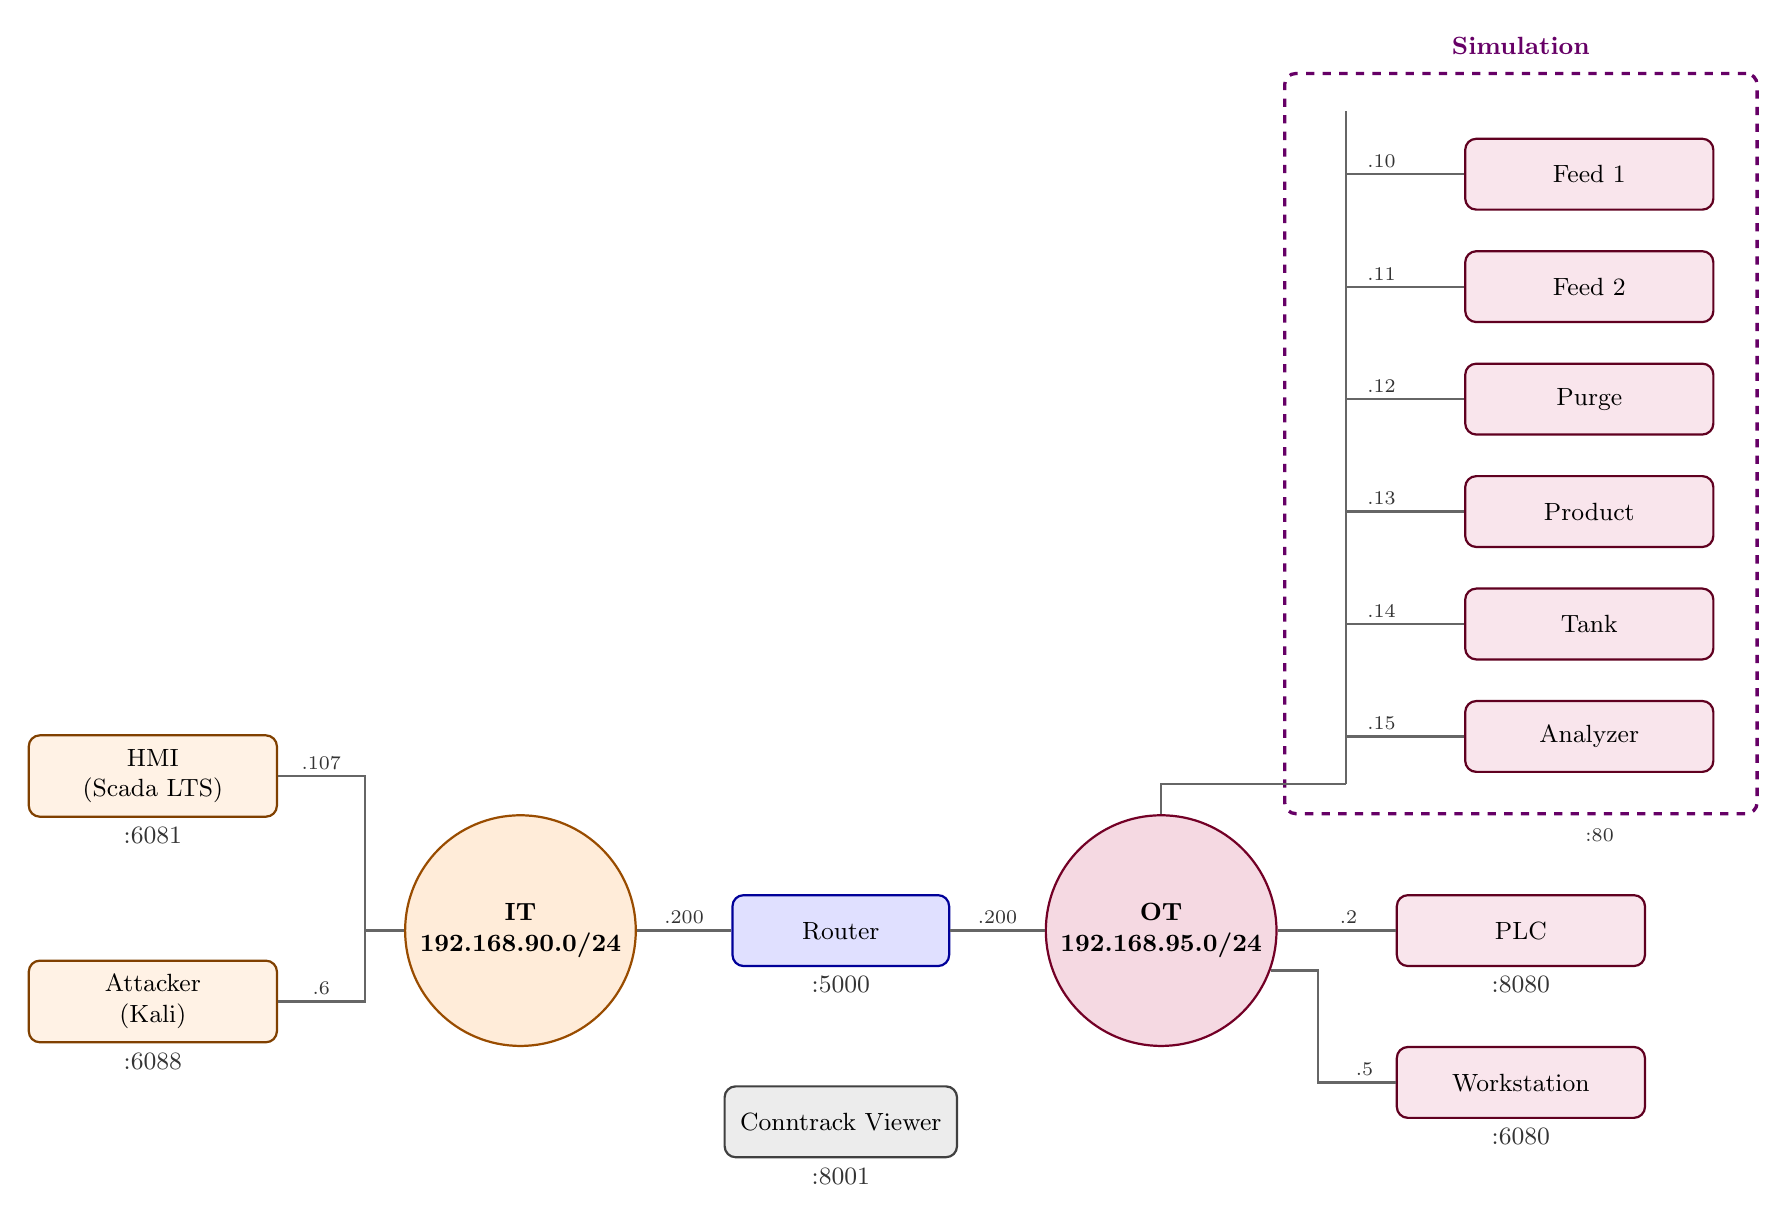
\begin{tikzpicture}[
    node distance=1.5cm and 1.2cm, 
    % --- BASE STYLES ---
    box/.style={rectangle, rounded corners, inner sep=5pt, align=center, font=\small, minimum height=0.9cm, text width=2.8cm, thick},
    hub/.style={circle, minimum size=2.8cm, align=center, font=\small\bfseries, thick},
    line/.style={draw=black!60, thick}, 
    iplabel/.style={font=\scriptsize, inner sep=2pt, text=black!80}, 
    node sub/.style={label={[font=\small, text=black!80]below:{#1}}},    
    % --- UNIFIED ZONE-BASED COLOR PALETTE ---
    % UNIFIED IT (AMBER ZONE)
    ithubnet/.style={hub, fill=orange!15, draw=orange!60!black},
    itnode/.style={box, fill=orange!10, draw=orange!50!black},    
    % BOUNDARY / DMZ (BLUE)
    boundarynet/.style={box, fill=blue!12, draw=blue!60!black, text width=2.4cm},    
    % NEUTRAL MONITOR (GRAY)
    monitornode/.style={box, fill=gray!15, draw=gray!50!black, text width=2.6cm},    
    % UNIFIED OT (PURPLE ZONE)
    othubnet/.style={hub, fill=purple!15, draw=purple!60!black},
    otnode/.style={box, fill=purple!10, draw=purple!50!black}
]

% ==========================================
% LEFT SIDE (UNIFIED AMBER IT ZONE)
% ==========================================
\node[itnode, node sub={:6081}] (hmi) {HMI\\(Scada LTS)};
\node[itnode, node sub={:6088}, below=1.8cm of hmi] (attacker) {Attacker\\(Kali)};
\node[ithubnet, right=1.6cm of attacker, yshift=0.9cm] (it_hub) {IT\\192.168.90.0/24};

% Clean right-angle bus for HMI and Attacker
\coordinate (it_in) at ($(it_hub.west) + (-0.5cm, 0)$);
\draw[line] (hmi.east) -- node[iplabel, above] {.107} (hmi.east -| it_in) -- (it_in);
\draw[line] (attacker.east) -- node[iplabel, above] {.6} (attacker.east -| it_in) -- (it_in);
\draw[line] (it_in) -- (it_hub.west);

% ==========================================
% MIDDLE (BLUE BOUNDARY & GRAY MONITOR)
% ==========================================
\node[boundarynet, node sub={:5000}, right=1.2cm of it_hub] (router) {Router};

% --- Conntrack Viewer (GRAY, RETURNED to original position) ---
% Positioned directly below the Router, showing its function as a central monitor.
\node[monitornode, node sub={:8001}, below=1.5cm of router] (conntrack) {Conntrack Viewer};

% Connections to Boundary elements
\draw[line] (it_hub.east) -- node[iplabel, pos=0.5, anchor=south] {.200} (router.west);
% Tapping point for the monitor at the boundary
% \draw[line] ($(router.west) + (0.5cm, 0)$) |- (conntrack.west);

% ==========================================
% RIGHT SIDE (UNIFIED PURPLE OT ZONE)
% ==========================================
\node[othubnet, right=1.2cm of router] (ot_hub) {OT\\192.168.95.0/24};
\draw[line] (router.east) -- node[iplabel, pos=0.5, anchor=south] {.200} (ot_hub.west);

% ==========================================
% OT DEVICES
% ==========================================
\node[otnode, node sub={:8080}, right=1.5cm of ot_hub] (plc) {PLC};
\node[otnode, node sub={:6080}, below=1cm of plc] (workstation) {Workstation};

\draw[line] (ot_hub.east) -- node[iplabel, pos=0.6, anchor=south] {.2} (plc.west);
\draw[line] (ot_hub.340) -- ++(0.6cm, 0) |- node[iplabel, pos=0.8, anchor=south] {.5} (workstation.west);

% ==========================================
% SIMULATION GROUP
% ==========================================
\node[draw=violet!80!black, 
      fill=white, 
      dashed, 
      rounded corners, 
      minimum width=6cm, 
      minimum height=9.4cm, 
      above=1cm of plc, 
      anchor=south, 
      very thick] (sim_group) {};

\node[font=\small\bfseries, text=violet!80!black, anchor=south, yshift=0.1cm] at (sim_group.north) {Simulation};
\node[iplabel, anchor=north] at ($(sim_group.south) + (1cm, -0.1cm)$) {:80};

% Bus Line 
\coordinate (sim_bus_top) at ($(sim_group.north west) + (0.8cm, -0.5cm)$);
\coordinate (sim_bus_bottom) at ($(sim_group.south west) + (0.8cm, 0.4cm)$); 
\draw[line] (sim_bus_top) -- (sim_bus_bottom);

% Simulation Nodes: Styles are set implicitly via otnode (purple zone)
\node[otnode, anchor=west] (feed1) at ($(sim_bus_top) + (1.5cm, -0.8cm)$) {Feed 1};
\node[otnode, anchor=west, below=0.5cm of feed1] (feed2) {Feed 2};
\node[otnode, anchor=west, below=0.5cm of feed2] (purge) {Purge};
\node[otnode, anchor=west, below=0.5cm of purge] (product) {Product};
\node[otnode, anchor=west, below=0.5cm of product] (tank) {Tank};
\node[otnode, anchor=west, below=0.5cm of tank] (analyzer) {Analyzer};

% Connect to bus
\foreach \n/\label in {feed1/.10, feed2/.11, purge/.12, product/.13, tank/.14, analyzer/.15} {
    \draw[line] (\n.west) -- node[iplabel, pos=0.7, anchor=south] {\label} (\n.west -| sim_bus_top);
}

% Connect OT Hub UP to the bus
\draw[line] (ot_hub.north) |- (sim_bus_bottom);

\end{tikzpicture}%
    }
    \caption{GRFICSv3 Network Diagram}
\end{figure}
Due to the safety and operational concerns discussed in~\ref{sec:data_lim_conf}, the reconnaissance attacks were not executed against the companies' OT environments. Instead, they were simulated in a virtual OT lab based on the open-source GRFICSv3 environment~\cite{grficsv3_2026}. GRFICSv3 is a containerized ICS/OT cyber-physical security lab that simulates an industrial chemical plant.

The attacks were run from the Kali attacker container (\texttt{192.168.90.6}) which, as shown in Figure~\ref{fig:env_diagram}, is located in the IT network. This represents the scenario where an attacker has obtained control over an IT-side host and performs reconnaissance towards the OT environment. The router/firewall container acts as the observation point, collecting all conntrack metadata form the crossing traffic

\textcolor{red}{the first stage of the Cyber Kill Chain (CKC)\cite{Yadav_2015}}. 

\subsection{Attack Scenarios}
The simulated attacks were designed to represent different forms of reconnaissance. The goal was to generate traffic patterns associated with host discovery, port discovery, service probing, and low-rate scanning. 

The scenarios vary in scan intensity and target scope. Some scans target the full OT subnet, while others target a smaller set of known live OT hosts. The full OT subnet corresponds to \texttt{192.168.95.0/24}. The selected live-host target set consists of known active hosts in the virtual OT network, including \texttt{192.168.95.2}, \texttt{192.168.95.5}, and
\texttt{192.168.95.10--192.168.95.15}. The simulated attacks are summarized in Table~\ref{tab:attack_scenarios}.

\begin{table}[h]
    
    \centering
    \caption{Overview of simulated reconnaissance attack types.}
    \label{tab:attack_scenarios}
    \makebox[\textwidth][c]{
    \begin{tabular}{lll}
        \hline
        Attack type & Scan configuration & Target scope \\
        \hline
        Aggressive subnet scan
            & \texttt{nmap -sS -Pn -T5 --top-ports 100}
            & Full OT subnet \\

        Fast subnet scan
            & \texttt{nmap -sS -Pn -T4 --top-ports 100/200}
            & Full OT subnet \\

        Default-speed subnet scan
            & \texttt{nmap -sS -Pn -T3 --top-ports 100}
            & Full OT subnet \\

        Slow subnet scan
            & \texttt{nmap -sS -Pn -T2 --top-ports 50/100}
            & Full OT subnet \\

        Very Slow targeted scan
            & \texttt{nmap -sS -Pn -T1 -p selected ports}
            & Selected live OT hosts \\

        Extremely slow targeted scan
            & \texttt{nmap -sS -Pn -T0 -p selected ports}
            & Selected live OT hosts \\

        Service/version detection
            & \texttt{nmap -sV -Pn -p selected ports}
            & Selected live OT hosts \\

        Host discovery
            & \texttt{nmap -sn}
            & Full OT subnet \\

        Low-and-slow scan
            & \texttt{nmap -sS -Pn -T2 --top-ports 50}
            & Full OT subnet \\
        \hline
    \end{tabular}
    }
\end{table}

For scanning nmap was selected because it is a widely used network scanning tool for host discovery, port scanning, and service identification, making it suitable for generating controlled reconnaissance traffic with configurable scan intensity and timing~\cite{nmap_nmap_nodate}. Most port discovery scenarios use TCP SYN scanning (\texttt{-sS}) with host discovery disabled (\texttt{-Pn}), so Nmap proceeds directly to probing the specified targets. The timing templates range from very aggressive (\texttt{-T5}) to extremely slow (\texttt{-T0}), allowing the dataset to include both faster and slower reconnaissance behavior. The low-and-slow scenario is included as an Advanced Persistent Threat (APT) inspired reconnaissance pattern, where probing activity is spread over a longer and interrupted period rather than concentrated in a short scan burst.

The selected port sets include common administrative and web ports such as
\texttt{22}, \texttt{80}, and \texttt{443}. They also include OT-relevant
services, most notably Modbus/TCP on port \texttt{502}. Modbus/TCP is commonly
used for supervision and control of automation equipment over TCP/IP networks,
and port \texttt{502} is frequently treated as the default Modbus/TCP port in
ICS scanning and measurement studies~\cite{ortega-fernandez_network_2024, cabana_detecting_2019}. In some runs, port \texttt{8080} was also included to cover web-based industrial interfaces.

Additional scenarios include host discovery (\texttt {-sn}), which identifies reachable devices in the target network without performing a full port scan. Service/version detection (\texttt{-sV}) is also performed as a later reconnaissance step where the scanner attempts to identify the applications or protocols running behind exposed ports\textcolor{red}~\cite{nmap_nmap_nodate}. 


\subsection{Attack Injection}
After executing the described reconnaissance attack scenarios, the adversarial traffic had to be isolated from the benign simulation traffic. This isolation was
based on the recorded attack timelines, the known attacker address, and the target scope of each scenario. Conntrack records were flagged as malign when their timestamps fell within the corresponding attack interval and their endpoints matched the expected bidirectional attacker-to-target communication. 

The isolated attack traces could not be directly inserted into the company data, since much of their metadata would not match. Specifically, the IP addresses and the timestamps from the virtual OT lab had to be modified in order to blend in. The IP remapping was deterministic, ensuring that attacker-side and target-side addresses were projected consistently onto IT-side and OT-side
company ranges, respectively. This preserves the intended attack direction of an IT host performing reconnaissance towards OT targets. The timestamps of the isolated attack traces were also shifted into the relevant periods of the company data. The relative timing within each attack was preserved, so that scan bursts, idle gaps, and low-and-slow patterns remained intact after injection.

After data remapping, the malicious data could be successfully injected into the validation and testing splits. Labels were assigned during this integration step. Original company traffic was treated as benign, while the injected reconnaissance records were labeled as malign traffic. The different attack names were also retained as metadata allowing us to later evaluate our results at a per attack scenario. 

It should be noted that while this is a good approximation of how reconnaissance attacks will look in the different customer environments, it does not fully reproduce all effects of an attack executed directly inside the companies' networks, such as device-specific responses, firewall behavior, or operational side effects.

\chapter{Detection Methodology}
\label{ch:detection_methodology}

% \section{Feature Engineering}
\section{Windowing}
The split, sorted and unidirectional labeled conntrack flows cannot be used directly for model training. Instead, they were aggregated into features representing flow properties over a fixed-length time windows in order to describe the communication behavior of each source host over time. 


Each model input is defined by a source IP address, a timestamp and a window length. In other words, all flows related to the same source host within that same time window are aggregated into one feature vector. For example, when using a 60-minute window, all flows associated with some source host \texttt{10.20.109.217} from 10:00 to 11:00 are combined into one vector containing features such as the number of contacted destination IPs, destination ports, protocol distribution, and packet or byte statistics. An example can be seen in Table~\ref{tab:feature_vector_preview}.

\begin{table}[htbp]
\centering
\caption{Example feature vectors after window-based aggregation.}
\label{tab:feature_vector_preview}
\small
\makebox[\textwidth][c]{%
\begin{adjustbox}{width=1.18\textwidth}
\begin{tabular}{lllrrrrrr}
\toprule
\texttt{src\_ip} & \texttt{win\_id} & \texttt{win\_start} &
\texttt{uniq\_dst} & \texttt{rx\_bytes} & \texttt{tx\_pkts} &
\texttt{mean\_B/pkt} & \texttt{mean\_dur\_s} \\
\midrule

10.20.109.217 & 492947 & 1774609200000 & 1 & 164 & 4 & 151.75 & 167.229 \\
% 1.24.16.14   & 492930 & 1774548000000 & 1 & 172 & 4 & 59.00  & 171.886 \\
% 1.83.125.119 & 492930 & 1774548000000 & 1 & 368 & 8 & 122.25 & 160.727 \\
% 1.83.125.25  & 493289 & 1775840400000 & 1 & 528 & 5 & 189.80 & 236.915 \\
% 1.83.125.35  & 492848 & 1774252800000 & 1 & 208 & 2 & 50.00  & 104.590 \\
\bottomrule
\end{tabular}
\end{adjustbox}%
}
\end{table}


A Prior work has shown that host‑level connection patterns are effective for traffic classification and anomaly detection, even when payloads are unavailable, traffic is unlabeled, or unidirectional\cite{dewaele_unsupervised_2010}. Similarly, as discussed \textcolor{red}{[IN LITERATURE  \cite{keshavamurthy_early_2023}]}, scanning behavior is usually visible as a change in the communication pattern of a source host (e.g. probing more ports), hence this kind of representation is highly suitable for reconnaissance. 

Feature extraction was performed on training, validation, and test splits for four different window sizes: \SI{60}{s}, \SI{300}{s}, \SI{3600}{s}, and \SI{18000}{s}, corresponding to one minute, five minutes, one hour and five hours respectively. Using multiple window sizes makes it possible to compare how detection performance changes when short bursts and longer low-rate reconnaissance activity are aggregated at different temporal resolutions.

\section{Features}
\label{sec:features}
\subsection{List of Features}
\label{sec:list_of_feat}


As discussed in \textcolor{red}{[the Related Work section]}, reconnaissance is an early-stage attack activity aimed at discovering reachable hosts, open ports, exposed services, and network structure. In network-flow metadata, this behaviour is expected to appear as a change in how a source host communicates. A scanning host may contact more destinations than usual, probe more destination ports, generate many short or low-volume connections, and receive fewer replies when targets are inactiveor closed. A list of features was chosen as a representation of this type of source behavior during the specified time window, and are displayed in Table~\ref{tab:feature_groups}. 



\begin{table}[htbp]
\centering
\scriptsize
\caption{Overview of extracted feature groups.}
\label{tab:feature_groups}
\renewcommand{\arraystretch}{2}
\begin{tabular}{
    >{\raggedright\arraybackslash}p{0.22\textwidth}
    >{\raggedright\arraybackslash}p{0.68\textwidth}
}
\toprule
Feature group & Features \\
\midrule
Window metadata
&
\texttt{ip\_src}, \texttt{window\_id}, \texttt{window\_start\_ts} \\

Volume
&
\texttt{flow\_count}, \texttt{total\_bytes}, \texttt{total\_packets},
\texttt{sent\_bytes}, \texttt{sent\_packets}, \texttt{received\_bytes},
\texttt{received\_packets} \\

Duration and packet statistics
&
\texttt{mean\_duration\_s}, \texttt{std\_duration\_s},
\texttt{mean\_bytes\_per\_packet}, \texttt{std\_bytes\_per\_packet},
\texttt{bytes\_per\_flow}, \texttt{packets\_per\_flow} \\

Destination and port diversity
&
\texttt{unique\_dst\_ip}, \texttt{unique\_dst\_port},
\texttt{unique\_src\_port}, \texttt{dst\_port\_per\_dst\_ip\_ratio} \\

Directionality and reply behavior
&
\texttt{outbound\_ratio}, \texttt{reply\_packet\_ratio},
\texttt{reply\_byte\_ratio}, \texttt{no\_reply\_packet\_score},
\texttt{no\_reply\_byte\_score}, \texttt{is\_pure\_upload\_like},
\texttt{is\_pure\_download\_like} \\

Entropy
&
\texttt{l4\_proto\_entropy}, \texttt{protocol\_entropy},
\texttt{ip\_src\_entropy\_window}, \texttt{ip\_dst\_entropy},
\texttt{port\_src\_entropy}, \texttt{port\_dst\_entropy},
\texttt{tcp\_src\_port\_entropy}, \texttt{tcp\_dst\_port\_entropy},
\texttt{udp\_src\_port\_entropy}, \texttt{udp\_dst\_port\_entropy} \\

TCP scan behavior
&
\texttt{tcp\_flow\_count}, \texttt{tcp\_short\_flow\_count},
\texttt{tcp\_short\_flow\_rate} \\

Temporal change
&
\texttt{flow\_count\_delta1}, \texttt{flow\_count\_mean3},
\texttt{unique\_dst\_ip\_delta1}, \texttt{unique\_dst\_ip\_mean3},
\texttt{unique\_dst\_port\_delta1}, \texttt{unique\_dst\_port\_mean3},
\texttt{tcp\_short\_flow\_rate\_delta1},
\texttt{tcp\_short\_flow\_rate\_mean3},
\texttt{no\_reply\_packet\_score\_delta1},
\texttt{no\_reply\_packet\_score\_mean3},
\texttt{ip\_dst\_entropy\_delta1}, \texttt{ip\_dst\_entropy\_mean3},
\texttt{port\_dst\_entropy\_delta1}, \texttt{port\_dst\_entropy\_mean3},
\texttt{outbound\_ratio\_delta1}, \texttt{outbound\_ratio\_mean3} \\
\bottomrule
\end{tabular}
\renewcommand{\arraystretch}{1.0}
\end{table}

\textcolor{blue}{should i bullet point these? or subsection them?}

The \textbf{window metadata} column identifies the source host and corresponding time window as supported by~\cite{dewaele_unsupervised_2010}.

\textbf{Volume features} describe the amount of communication associated with a source host. They include \feat{flow\_count}, \feat{total\_bytes}, \feat{total\_packets}, \feat{sent\_bytes}, \feat{sent\_packets}, \feat{received\_bytes}, and \feat{received\_packets}. These features capture whether a host becomes more active than usual and whether the activity is mainly outgoing, incoming, or
balanced. Similar flow-based anomaly detection systems are described by Dromard~\cite{dromard_online_2017}, who also relies on sliding‑window statistics to capture abrupt deviations in traffic behavior.

% The \textbf{flow duration and packet statistics} features describe the shape of the flows rather than only their total volume. Reconnaissance traffic often consists of many lightweight connection attempts, so features such as \feat{mean\_duration\_s}, \feat{std\_duration\_s}, \feat{mean\_bytes\_per\_packet}, \feat{bytes\_per\_flow}, and \feat{packets\_per\_flow} can help distinguish short probing behavior from regular communication.

\textbf{Flow duration and packet statistics} describe another dimension of network behavior. Features such as \feat{mean\_duration\_s} and \feat{std\_duration\_s} summarize how long the observed flows last, while \feat{mean\_bytes\_per\_packet}, \feat{std\_bytes\_per\_packet}, \feat{bytes\_per\_flow}, and \feat{packets\_per\_flow} describe how much traffic is exchanged per flow and per packet. These features are relevant for reconnaissance traffic which may produce many short and lightweight connections, especially during host or port probing. Similar features are included in standard NetFlow based feature sets for network intrusion detection~\cite{Sarhan_2021}

The \textbf{destination and port diversity} features capture how widely a source host communicates within a time window. \texttt{unique\_dst\_ip} measures the number of distinct destinations contacted, while \texttt{unique\_dst\_port}, \texttt{unique\_src\_port}, and \texttt{dst\_port\_per\_dst\_ip\_ratio} describe the diversity of contacted services and ports. These features are directly relevant to reconnaissance, because horizontal scans contact many hosts, vertical scans contact many ports on one host, and mixed scans may affect both dimensions~\cite{ring_detection_2018}.

The \textbf{directionality and reply-behavior} features are included to capture whether a source host mainly initiates communication and whether those attempts receive substantial responses. Features such as \feat{outbound\_ratio}, \texttt{reply\_packet\_ratio}, \texttt{reply\_byte\_ratio}, \texttt{no\_reply\_packet\_score}, and \texttt{no\_reply\_byte\_score} are especially useful for scan-like behavior, where probes may be sent towards closed ports, inactive hosts, filtered targets, or services that do not exist~\cite{ring_detection_2018}.

The \textbf{TCP scan behavior} features focus on TCP-specific probing. Since many of the simulated reconnaissance scenarios use TCP SYN scanning, the number and fraction of short TCP flows are included as indicators of incomplete or unsuccessful TCP connection attempts. In a SYN scan, the attacker sends the initial SYN request and typically does not complete the three-way handshake for open ports~\cite{ring_detection_2018}.

The \textbf{entropy} features summarize how concentrated or dispersed communication is. Low entropy indicates that most traffic is concentrated on a small number of values, while higher entropy indicates a more diverse distribution. For a categorical feature $X$ with possible observed values $v_i$, the Shannon entropy is computed as:
\[
H(X) = - \sum_{i=1}^{m} p(v_i)\log_2 p(v_i),
\]
where $p(v_i)$ is the relative frequency of value $v_i$ in the considered source-host window, and $m$ is the number of distinct observed values. For example, \feat{port\_dst\_entropy} is computed from the distribution of destination ports contacted by a source host in a window, while \feat{ip\_dst\_entropy} is computed from the distribution of contacted destination IP addresses. A host that repeatedly communicates with one service has lower destination-port entropy than a host whose traffic is spread across many ports, which can indicate scanning behavior. Cai et al. uses these exact features in their proposed ADAM scheme, which makes up one of the tested models in this thesis as discussed in Section~\ref{sec:ADAM}.

Finally, the \textbf{temporal change features} describe how specific behavioral features evolve across consecutive windows. The \texttt{\_delta1} features measure the change relative to the previous window for the same source host, while the \texttt{\_mean3} features compute a short rolling average over the current and two previous windows.  The three-window average provides limited temporal smoothing without aggregating behavior over too long a period. These features are included because slow reconnaissance may not produce a strong anomaly in a single isolated window, but may become more visible over time~\cite{ring_detection_2018}.

A more detailed explanation of each feature can be found in Appendix~\ref{app:feature_descriptions}.

\subsection{Feature Sets}



Feature sets were constructed using an iterative selection process, by comparing the defined features from Section~\ref{sec:list_of_feat} of the benign and malign data. For each feature, benign and malign validation windows were compared using their mean and median values. For each feature $f$, the benign mean $\mu_b$, malicious mean $\mu_m$, benign standard deviation $\sigma_b$, and malicious standard deviation $\sigma_m$ were computed. To rank features in a scale-independent way, the difference between the benign and malicious means was normalized by the pooled standard deviation, resulting in a Cohen's d  standardized mean difference~\cite{lakens_calculating_2013}.
\[
\sigma_{\mathrm{pooled}} =
\sqrt{\frac{\sigma_b^2 + \sigma_m^2}{2}},
\]

resulting in the standardized mean difference

\[
\mathrm{SMD}(f) =
\frac{\mu_m - \mu_b}{\sigma_{\mathrm{pooled}}}.
\]

Features were ranked by $|\mathrm{SMD}(f)|$, so that features with different numerical scales could be compared fairly and features were ranked highly regardless of whether they increased or decreased during attacks. Median differences were also inspected to make the ranking easier to interpret for possible skewed features. This comparison was repeated for each different time window (\SI{60}{s}, \SI{300}{s}, \SI{3600}{s}, and \SI{18000}{s}) and for each different attack category grouped by intensity (T0/T1, T2, T3/T4/T5). As an indicator, Table~\ref{tab:global_feature_ranking} captures a global ranking of feature importance, combining all of the different window, attack combinations.




\begin{table}
\caption{Global feature ranking based on the median absolute standardized mean difference across attack/window-specific rankings.}
\label{tab:global_feature_ranking}
\begin{tabular}{r l r r}
\toprule
Rank & Feature & Median |SMD| & Mean |SMD| \\
\midrule
1 & ip\_dst\_entropy\_mean3 & 7.046000 & 7.026000 \\
2 & ip\_dst\_entropy & 6.704000 & 6.773000 \\
3 & tcp\_short\_flow\_rate\_mean3 & 6.246000 & 5.608000 \\
4 & tcp\_short\_flow\_rate & 6.215000 & 5.573000 \\
5 & unique\_dst\_ip\_mean3 & 3.511000 & 9.212000 \\
6 & no\_reply\_packet\_score\_mean3 & 2.942000 & 3.101000 \\
7 & no\_reply\_packet\_score & 2.922000 & 3.088000 \\
8 & unique\_dst\_ip & 2.801000 & 8.598000 \\
9 & is\_pure\_upload\_like & 2.294000 & 2.407000 \\
10 & outbound\_ratio\_mean3 & 2.273000 & 2.363000 \\
% 11 & outbound\_ratio & 2.263000 & 2.356000 \\
% 12 & is\_pure\_download\_like & 2.210000 & 2.296000 \\
% 13 & tcp\_short\_flow\_count & 2.014000 & 24.566000 \\
% 14 & no\_reply\_byte\_score & 1.887000 & 1.757000 \\
% 15 & reply\_packet\_ratio & 1.570000 & 1.433000 \\
% 16 & ip\_src\_entropy\_window & 1.294000 & 1.143000 \\
% 17 & port\_dst\_entropy & 0.840000 & 0.805000 \\
% 18 & port\_dst\_entropy\_mean3 & 0.832000 & 0.770000 \\
% 19 & tcp\_dst\_port\_entropy & 0.805000 & 0.814000 \\
% 20 & dst\_port\_per\_dst\_ip\_ratio & 0.766000 & 0.777000 \\
\bottomrule
\end{tabular}
\end{table}



\begin{figure}[htbp]
    \centering

    \begin{adjustbox}{width=1.4\textwidth, center}
        \begin{minipage}{1.4\textwidth}
            \centering

            \begin{minipage}{0.49\textwidth}
        \centering
        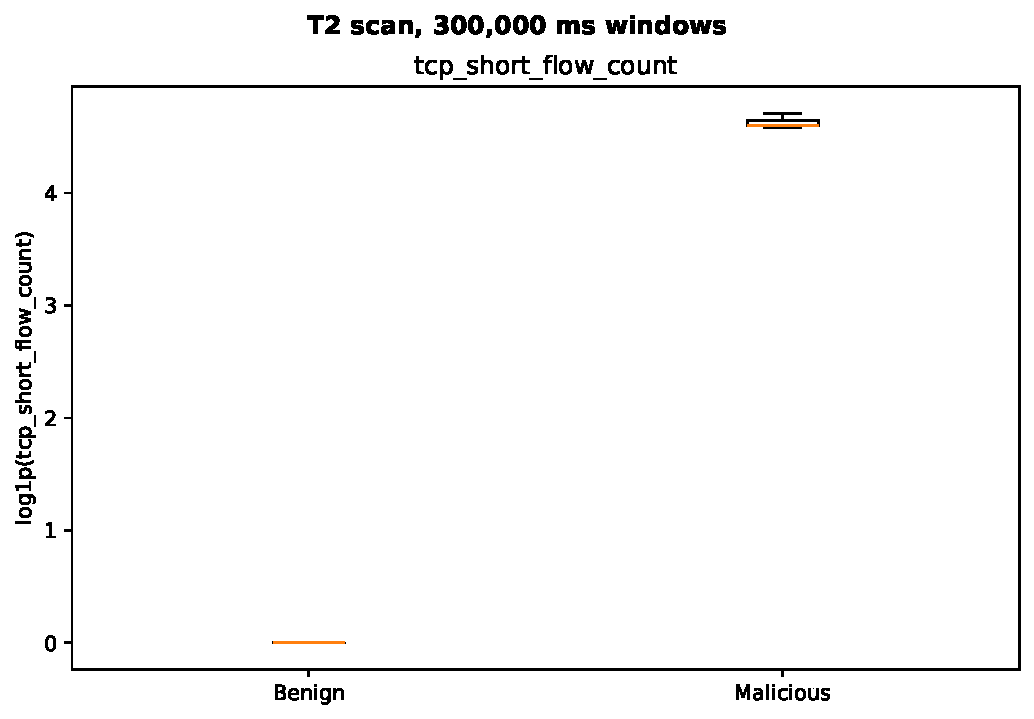
\includegraphics[width=\linewidth]{figures/boxplots_t2_scan_300000ms.pdf}
        \small (a) 
    \end{minipage}
    \hfill
    \begin{minipage}{0.49\textwidth}
        \centering
        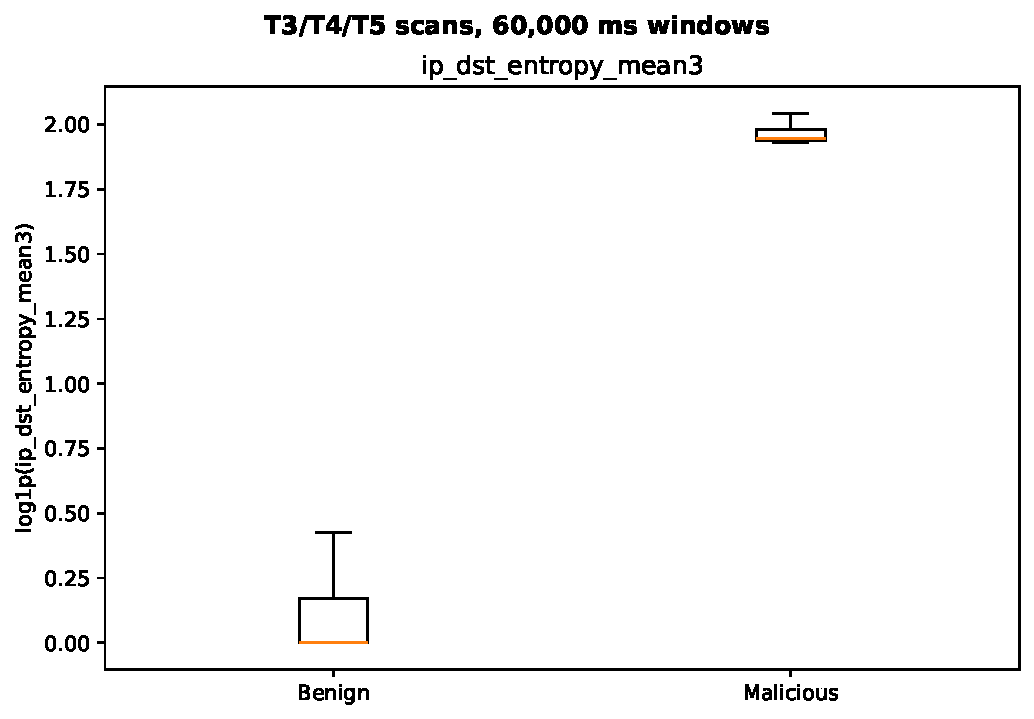
\includegraphics[width=\linewidth]{figures/boxplots_t3_t4_t5_scans_60000ms.pdf}
        \small (b) 
    \end{minipage}


        \end{minipage}
    \end{adjustbox}
    \captionsetup{width=1.3\textwidth}
    \caption{Benign--malicious boxplot comparisons for selected reconnaissance-related features. 
(a) \texttt{tcp\_short\_flow\_count} for the T2 attack using 5-minute windows. 
(b) \texttt{ip\_dst\_entropy\_mean3} for the T3/T4/T5 attacks using 1-minute windows. 
}
    \label{fig:selected_feature_boxplots}
\end{figure}

The ranked summaries of each attack group and window, were used to identify feature families that consistently distinguished reconnaissance from benign traffic. Some of the strongest recurring features were \feat{ip\_dst\_entropy} and \feat{ip\_dst\_entropy\_mean3} representing destination spread, \feat{tcp\_short\_flow\_rate} and \feat{tcp\_short\_flow\_rate\_mean3} representing short-lived TCP scan behavior, and \feat{no\_reply\_packet\_score} and \feat{outbound\_ratio} representing failed or asymmetric communication. Two of these features are illustrated as boxplots in Figure~\ref{fig:selected_feature_boxplots}, visualizing the separation. Based on this information, candidate feature sets were constructed to cover multiple aspects of reconnaissance behavior while limiting redundancy between strongly related features.

This resulted in three types of feature sets. First, general-purpose sets, combining the strongest non-redundant features. Second, attack specific sets emphasizing particular behavior, such as fast and broad scans, stealthy and slow scans, or horizontal host discovery. The last type, isolated specific signal families, such as entropy-only (ADAM), or asymmetry-only groups to get more information on which underlying reconnaissance behaviors contributed most to detection. It is important to clarify that the test split was not used during this feature-set construction process in order to avoid leakage. The exact feature sets can be observed in~\ref{app:feature_sets}.


\section{Anomaly Detection Models}
All models in this section are evaluated in a one-class anomaly detection setting. During training, the models do not rely on labeled data as they are only trained on benign windows, learning a reference of what normal traffic in a specific environment looks like and assigning an anomaly score to unseen windows based on their deviation from this benign reference. Ground-truth labels are introduced only after scoring, in order to evaluate performance.

\subsection{k-Nearest Neighbors}
As discussed in Section [LITERATURE REVIEW], k-Nearest Neighbors (k-NN) is traditionally a supervised learning algorithm, where a new sample is classified based on the labels of its closest neighbors in the training data. However, the same distance-based principle can also be used for one-class anomaly detection.  In that case,the training phase does not involve learning model weights. Instead, the model stores the benign training observations in the selected feature space. During evaluation, each new sample is compared to these stored benign observations using a distance metric. If the sample is close to previously observed normal behavior, it receives a low anomaly score. If it is far from the benign reference set, it receives a high anomaly score. A threshold is then used to decide when this distance is large enough for the window to be considered anomalous.

This principle is reflected in our implementation. The k-NN model is fitted only on the benign training split for which training data is first sorted chronologically by \texttt{window\_start\_ts} and \texttt{window\_id}. The first 80\% of the sorted benign training data is used to build the nearest-neighbor reference set, while the remaining 20\% is kept aside for threshold calibration. This calibration subset is still benign, but is not used to fit the k-NN model itself. After fitting, the model is applied to the calibration subset to estimate the range of distance scores that can still occur under normal behavior. Different percentile thresholds are then tested based on this benign score distribution.

Features are scaled using \texttt{RobustScaler}~\cite{pedregosa_scikit-learn_nodate}, which is fitted only on the 80\% reference subset and then applied unchanged to the calibration and evaluation data. This scaler centers each feature around its median and scales it according to the interquartile range, meaning the spread between the 25th and 75th percentiles. Robust scaling was chosen because derived features may contain extreme values even in benign traffic, the effect of which is contained with this method. The nearest-neighbor search is implemented using the \texttt{NearestNeighbors} class from \texttt{scikit-learn}~\cite{pedregosa_scikit-learn_nodate}, configured with Euclidean distance. Meira et al. empirically validated the use of standard Euclidean distance as the core distance metric when successfully applying One-Class Nearest Neighbor algorithms to network intrusion detection datasets~\cite{meira_performance_2020}. For each input sample, the distances to the \(k\) nearest benign reference samples is computed, by averaging the score to this \(k\) nearest neighbors.
\subsubsection{ADAM}
\label{sec:ADAM}
An additional k-NN variant was included for evaluation based on the feature representation proposed in ADAM. ADAM combines entropy-based traffic profiling with unsupervised anomaly detection for DDoS mitigation in software-defined cyber-physical systems. Normal traffic is represented using entropy based features over the network and transport layer, and it selects k-NN as the anomaly detection modules because of its balance between time overhead and detection affectiveness~\cite{cai_adam_2023}. In order to evaluate the effectiveness of the ADAM proposed feature set, some experiments were run exclusevily using features form the Entropy group in Table~\ref{tab:feature_groups}.



\subsection{Outlier-aware Denoising Autoencoder}
The next anomaly detection approach is based on the the CPS-GUARD method, which uses a semi-supervised deep autoencoder together with an outlier aware threshold selection procedure~\cite{catillo_cps-guard_2023}. Autoencoders are neural networks trained to reconstruct their own input. In anomaly detection, the underlying assumption is that the model trained on benign data will learn to reconstruct normal behavior well, while windows that differ from this learned normal behavior will result in a larger reconstruction error. This error can therefore be used as an anomaly score.

The model is again trained only on benign training windows. The selected input features are first scaled using a preprocessing pipeline consisting of \texttt{RobustScaler} followed by \texttt{MinMaxScaler} with a target range of \([-1,1]\). Robust scaling is used to reduce the influence of extreme feature values, while the min-max scaling step matches the range of the autoencoder output layer, which uses a \texttt{tanh} activation function.

The autoencoder follows a symmetric encoder-decoder structure. Several architectures are evaluated, including the original CPS-GUARD-style \(N\)-36-6-36-\(N\) architecture but also larger or smaller variants, where \(N\) is the number of selected input features. In this notation, \(N\) denotes the number of selected input features. The architecture therefore maps an \(N\)-dimensional input vector to a first hidden layer with 36 neurons, compresses it to a 6-neuron bottleneck representation, expands it again to 36 neurons, and finally reconstructs an \(N\)-dimensional output vector. The hidden layers use ReLU activations, while the output layer uses \texttt{tanh}.The model is trained with mean squared error as reconstruction loss and RMSProp as optimizer. To reduce overfitting to the benign training windows, dropout is applied after the first two hidden layers, as well as Gaussian input noise as a regularization mechanism. A diagram of this model initialized with \(N\)-36-6-36-\(N\) architecture is depicted in Figure~\ref{fig:cpsguard_autoencoder_architecture}

\begin{figure}[htbp]
\centering
\begin{adjustbox}{width=\textwidth}
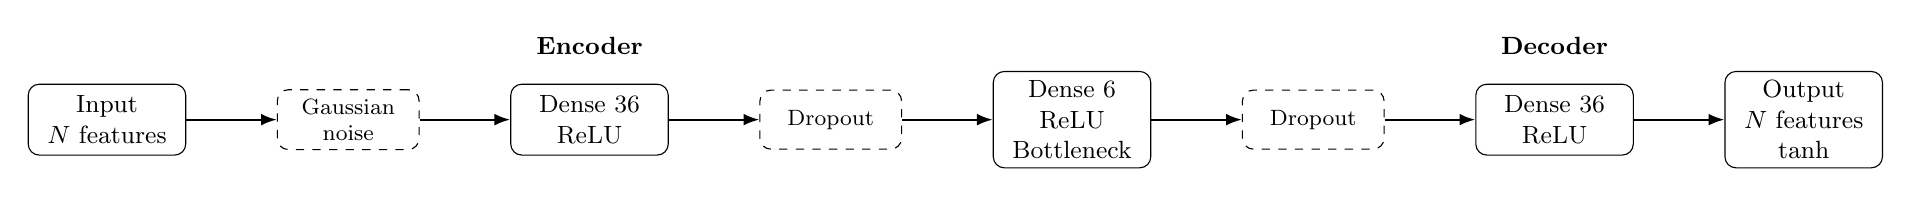
\begin{tikzpicture}[
    node distance=1.15cm,
    every node/.style={font=\small},
    layer/.style={
        draw,
        rounded corners,
        align=center,
        minimum width=2.0cm,
        minimum height=0.9cm
    },
    reg/.style={
        draw,
        dashed,
        rounded corners,
        align=center,
        minimum width=1.8cm,
        minimum height=0.75cm,
        font=\footnotesize
    },
    arrow/.style={-{Latex[length=2mm]}, thick}
]

\node[layer] (input) {Input\\$N$ features};
\node[reg, right=of input] (noise) {Gaussian\\noise};
\node[layer, right=of noise] (enc1) {Dense 36\\ReLU};
\node[reg, right=of enc1] (drop1) {Dropout};
\node[layer, right=of drop1] (bottleneck) {Dense 6\\ReLU\\Bottleneck};
\node[reg, right=of bottleneck] (drop2) {Dropout};
\node[layer, right=of drop2] (dec1) {Dense 36\\ReLU};
\node[layer, right=of dec1] (output) {Output\\$N$ features\\tanh};

\draw[arrow] (input) -- (noise);
\draw[arrow] (noise) -- (enc1);
\draw[arrow] (enc1) -- (drop1);
\draw[arrow] (drop1) -- (bottleneck);
\draw[arrow] (bottleneck) -- (drop2);
\draw[arrow] (drop2) -- (dec1);
\draw[arrow] (dec1) -- (output);

\node[above=0.25cm of enc1] {\textbf{Encoder}};
\node[above=0.25cm of dec1] {\textbf{Decoder}};

\end{tikzpicture}
\end{adjustbox}
\caption{CPS-GUARD-style autoencoder architecture used for reconstruction-based anomaly detection. The \(N\)-dimensional feature vector is regularized using Gaussian noise, compressed into a lower-dimensional bottleneck representation, and then reconstructed at the output. Dropout is applied after the first two hidden layers during training.}
\label{fig:cpsguard_autoencoder_architecture}
\end{figure}

For threshold selection, the benign training data is divided into an autoencoder training subset and a separate benign threshold-calibration subset, which is excluded from training. After training, the calibration subset is passed through the autoencoder and each calibration window receives a reconstruction error, which represents a range of scores that can still occur at benign inputs. Then Isolation Forest is applied to the calibration subset to separate benign calibration samples from outliers~\cite{catillo_cps-guard_2023}. The reconstruction errors of these two groups are used by the threshold selection procedure to choose a final anomaly threshold. This way, instead of directly selecting a fixed percentile of all benign reconstruction errors, possible outliers in the benign calibration set are filtered out. Different contamination values were tested for this step.



\subsection{K-means}
The final model used is based on K-means clustering. K-means is an unsupervised clustering algorithm that partitions the training data into \(k\) clusters by assigning samples to the nearest cluster centroid. Although K-means is primarily a clustering algorithm, it can be adapted to one-class anomaly detection by treating the distance to the nearest benign cluster centroid as an anomaly score~\cite{meira_performance_2020}. Then, during evaluation, a new sample is compared to these centroids. Samples close to one of the benign clusters receive a low anomaly score, while samples far away from all learned centroids receive a high anomaly score.

As repeated for the previous models, the K-means model is fitted only on the benign training split. The training data is first sorted chronologically by \feat{window\_start\_ts} and, \feat{window\_id} of which the first 80\%  is used to fit the K-means model, while the remaining 20\% is kept aside as a benign calibration subset for threshold selection. Features are scaled using \feat{RobustScaler}, which is fitted only on the 80\% model-fitting subset and then applied unchanged to the calibration and evaluation data.

After training, each calibration sample is assigned an anomaly score equal to its Euclidean distance to the nearest cluster centroid. The anomaly threshold is then selected as a tested quantile of these benign calibration distances. During evaluation, each validation or test window is scaled using the same scaler and assigned its nearest-centroid distance. A window is classified as anomalous when this distance exceeds the selected threshold.

Several values for the number of clusters are tested. Smaller values force the model to represent benign behavior using only a few broad traffic profiles, while larger values allow the model to capture more fine-grained modes of normal behavior. Similarly to the k-NN approach, different threshold quantiles are evaluated to study the trade-off between detecting malicious windows and limiting false positives on benign traffic.  The implementation uses the \texttt{MiniBatchKMeans} class from \texttt{scikit-learn}~\cite{pedregosa_scikit-learn_nodate}.




% talk about the zscore and why we don't use it.




\section{Experimental Configuration}
With the defined models, there are still several design choices that can influence their detection performance. These include the feature set, aggregation window length, anomaly threshold, and model-specific parameters such as the number of nearest neighbors, number of K-means clusters, autoencoder architecture, and Isolation Forest contamination value. In order  to meaningfully select the model that would best perform for reconnaissance detection on conntrack-derived OT traffic, all possible combination of these parameters were explored. 

The sweeps are organized around four main dimensions. First, multiple aggregation window sizes are evaluated in order to study how temporal granularity affects detection. Shorter windows may capture short scanning bursts more precisely, while longer windows may smooth traffic behavior and make low-rate reconnaissance activity more visible. Second, several feature sets are tested, ranging from more general reconnaissance based sets, to more case specialized sets as discussed in~\ref{sec:features}. Third, each model is evaluated under multiple threshold settings. For distance-based models (such as K-NN or K-means), thresholds are selected as quantiles of the benign calibration score distribution, and for the autoencoder different Isolation Forest contamination values are tested. Finally, model-specific parameters are varied, such as \(k\) for k-NN, the number of clusters for K-means, and the hidden-layer dimensions of the autoencoder.

After exploring all these possibilities, the validation data is used to evalute which configurations show the most promising results. Based on this parameters are modified as suited and certain feature sets are added or removed for the next sweeps. The validation data is also used to select the best model/parameter combinations to be advanced to the testing phase.

\section{Evaluation Metrics}



The models are evaluated using both window-level and range-lavel metrics. Window-level F1 treats each window independently which can be limiting for reconnaissance detection, because an attack is usually not a single isolated window, but an activity that unfolds over a continuous time interval. A detector that raises at least one alarm during such an interval may already be useful from an operational perspective, even if it does not flag every malicious window. Similarly, a model may obtain a good window level F1-score while producing several separate false alarm intervals, which would be less desirable for an operator. This issue is also discussed by Fung et al.~\cite{atluri_perspectives_2022} , who show that point-wise F1 can give a misleading impression of anomaly detection performance in ICS time-series settings, and argue that range-based metrics better capture operational objectives such as reducing false alarms and detecting attack intervals.

Window-level precision, recall and F1-score are computed from the number of true positives, false positives and false negatives over all evaluated windows. A true positive (TP) is a window that overlaps with an attack interval and is predicted as anomalous. A false positive (FP) is a benign window that is incorrectly predicted as anomalous, while a false negative (FN) is an attack window that is not detected. These metrics provide a more fine grained view and are useful for comparing how precisely each model identifies anomalous windows. 

For the discussed range based precision, recall and F1-score, the true labels and model predictions are first processed separately for each source host. Consecutive positive windows are grouped into temporal ranges after sorting by timestamp. A true attack range is counted as detected when at least one predicted anomalous range overlaps with it. Predicted anomalous ranges that do not overlap with any true attack range are counted as range-level false positives, while true attack ranges without any overlapping prediction are counted as range-level false negatives. Hence, the range-based metric used here therefore follows an event-detection interpretation. It does not require every malicious window inside an attack interval to be classified correctly.


Window-level precision, recall and F1-score are defined as:

\begin{equation}
    \text{Precision} = \frac{TP}{TP + FP}
\end{equation}

\begin{equation}
    \text{Recall} = \frac{TP}{TP + FN}
\end{equation}

\begin{equation}
    F_1 = 2 \cdot \frac{\text{Precision} \cdot \text{Recall}}
    {\text{Precision} + \text{Recall}}
\end{equation}

where \(TP\), \(FP\), and \(FN\) are counted over individual source-host windows.


The same precision, recall and F1-score definitions are then applied at the range level:



\begin{equation}
    \text{Range Precision} = 
    \frac{TP_{\text{range}}}{TP_{\text{range}} + FP_{\text{range}}}
\end{equation}

\begin{equation}
    \text{Range Recall} = 
    \frac{TP_{\text{range}}}{TP_{\text{range}} + FN_{\text{range}}}
\end{equation}

\begin{equation}
    F_{1,\text{range}} =
    2 \cdot
    \frac{\text{Range Precision} \cdot \text{Range Recall}}
    {\text{Range Precision} + \text{Range Recall}}
\end{equation}

A predicted range \(P=[p_s,p_e]\) overlaps a true attack range \(T=[t_s,t_e]\) when:
\[
p_s \leq t_e \land p_e \geq t_s .
\]

Both metrics are reported because they provide complementary views of the same predictions. Window-level F1 evaluates each source-host window separately, while range-level F1 summarizes consecutive detections into temporal alarm ranges. Differences between them are therefore interpreted as different perspectives on model performance, rather than as contradictory results.





% 3.6 Anomaly Detection Models
%     3.6.1 KNN-Based Detector
%     3.6.2 Isolation Forest
%     3.6.3 Deep Autoencoder + Isolation Forest
%     3.6.4 ADAM-Inspired Statistical Baseline
%     3.6.5 Optional: K-Means Baseline

% 3.7 Threshold Selection and Hyperparameter Tuning

% 3.8 Evaluation Metrics
% SINCE we are aggragatng features we are already doing a knd of range based metric but here then the range based is for the entre range of the attack.
%     3.8.1 Point-Based Metrics
%     3.8.2 Range-Based Metrics
%     3.8.3 Comparison Between Metric Types

% 3.9 IT Comparison Dataset

% 3.10 Implementation Details and Reproducibility
%   -dask
% \include{chapter-1}
% % ... and so on until
\chapter{Results}
% - results and discussion
% - compare models and hyperparameters and feature sets and windows and attacks (easy vs stealthy performance)
% - And how it compares to IT


% plot correlation between parameters and certain feature sets and window lengthS?

% if an attacker could spend some time in the network they could observe the packets and try to match the metatada of his attack as much as possible

% possible big difference between test and val because of the misconfigurations in validation data.

\section{Evaluation Overview}
% Briefly explain models, splits, metrics and how to read the results.
\textcolor{blue}{is this too much repetition?}


This chapter presents the experimental results of the evaluated anomaly detection
models on the constructed reconnaissance detection datasets. The goal of the
evaluation is to determine to what extent unsupervised models trained only on
benign conntrack-derived traffic can detect injected reconnaissance activity in
real OT background traffic. As described in Section~\ref{sec:experimental_configuration}, the configurations vary in feature set, aggregation window length, anomaly threshold, and model-specific parameters.
For k-NN, the search space is more limited than for K-Means and the autoencoder
because of its higher computational cost. The k-NN results are therefore
interpreted as a targeted evaluation of validation-selected feature sets rather
than as a full sweep over all candidate feature sets.


The experiments are evaluated in two stages. First, the validation split is used
to compare configurations and identify promising model, feature-set and parameter
combinations. These validation results are used for model selection and for
understanding the effect of design choices such as window size and feature
selection. The selected configurations are then evaluated on the test split, which
is kept separate from the selection process and is used to assess how well the
chosen configurations generalize to another period of network traffic.

The results are reported using both window-level and range-level metrics.
Window-level metrics treat each source-host window as an individual prediction
and therefore measure how accurately the model classifies separate time windows.
Range-level metrics instead group consecutive anomalous windows into alarm
ranges and compare these ranges with the true attack intervals. This provides a
more operational view of the results, since reconnaissance activity usually
unfolds over a period of time rather than in a single isolated window.

Both views are used throughout the discussion. Window-level F1 indicates how
precise the model is at the individual-window level, while range-level F1
indicates whether complete reconnaissance scenarios are detected as temporal
events and how many separate false alarm ranges are produced. A model may
therefore have a moderate window-level score while still detecting the relevant
attack interval, or a strong window-level score while producing fragmented
alarms.

Unless stated otherwise, the tables in this chapter report configurations selected
according to validation performance, followed by their corresponding test-set
performance. Differences between validation and test results are interpreted as an
indication of robustness and sensitivity to the underlying benign traffic period.



\section{Validation-Based Feature Set Selection}
\label{sec:validation_feature_selection}
% Show top validation feature sets, explain reduced k-NN search.

Before comparing the final model configurations on the test split, the validation results were used to identify the most promising feature sets. This step was especially important because the full feature-set search could not be repeated exhaustively for k-NN due to its higher computational cost, as discussed in Section~\ref{sec:knn_resource_constraints}. The selection was therefore based on the full K-Means and autoencoder validation sweeps, which covered the complete planned feature-set space. 

\definecolor{selectedrow}{RGB}{230,242,255}

\
\begin{table}[htbp]
\centering
\small
\renewcommand{\arraystretch}{1.25}
\setlength{\tabcolsep}{3.5pt}
\makebox[\textwidth][c]{%
\begin{tabularx}{1.05\textwidth}{>{\raggedright\arraybackslash}X l l l l}
\toprule
Feature set & \#configs & Mean RF1 & Mean F1 & Score \\
\midrule

\rowcolor{selectedrow}
\feat{golden\_minimal} 
& 896 & 0.224 & 0.261 & 0.242 \\

\rowcolor{selectedrow}
\feat{omni\_core\_clean} 
& 896 & 0.214 & 0.250 & 0.232 \\

\feat{adam\_entropy} 
& 336 & 0.183 & 0.225 & 0.204 \\

\rowcolor{selectedrow}
\feat{low\_slow\_clean} 
& 896 & 0.127 & 0.157 & 0.142 \\

\feat{T2\_stealth\_scan} 
& 896 & 0.099 & 0.116 & 0.107 \\

\feat{T3\_T4\_T5\_loud\_scan} 
& 896 & 0.116 & 0.085 & 0.101 \\

\feat{recon\_core\_clean\_temporal} 
& 896 & 0.075 & 0.090 & 0.083 \\

\feat{ablation\_entropy\_only} 
& 896 & 0.061 & 0.050 & 0.055 \\

\feat{recon\_core\_clean} 
& 896 & 0.050 & 0.059 & 0.054 \\

\feat{horizontal\_scan\_clean} 
& 336 & 0.072 & 0.035 & 0.054 \\

\feat{ablation\_asymmetry\_only} 
& 336 & 0.000 & 0.000 & 0.000 \\

\bottomrule

\end{tabularx}
}
\caption{Validation-based feature set ranking. RF1 denotes range-level F1, and \#configs is the number of validation configurations included for each feature set. The selection score is computed as the average of mean validation RF1 and mean validation window-level F1. Highlighted rows indicate the feature sets selected for the final cross-model comparison and targeted k-NN evaluation.}
\label{tab:validation_feature_set_ranking}
\end{table}



The goal of this selection was not only to find the highest individual validation score, but to identify feature sets that performed well across multiple reconnaissance scenarios. Feature sets that were designed for one specific attack type were therefore interpreted with caution, even when they achieved strong results on that specific attack. Instead, preference was given to feature sets with broader coverage across the evaluated attacks. To summarize the validation results across feature sets, a compact selection score is used. This score gives equal weight to the mean validation range F1 and the mean validation window-level F1. Table~\ref{tab:validation_feature_set_ranking} shows the resulting ranking. 


The number of configurations is not identical for all feature sets. The general-purpose feature sets were included in the full K-Means and autoencoder validation sweeps. In contrast, \feat{csv\_adam\_entropy} was evaluated as an ADAM-inspired k-NN baseline and therefore has fewer configurations. It will be further discussed in Section~\ref{sec:adam_baseline}. Similarly, \feat{csv\_horizontal\_scan\_clean} and \feat{csv\_ablation\_asymmetry\_only} were dropped earlier based on their weaker validation behavior, so their scores are based on a smaller set of configurations. 

The two strongest feature sets are \feat{csv\_golden\_minimal} and \feat{csv\_omni\_core\_clean}, which both achieve the highest combined validation scores. \feat{csv\_low\_slow\_clean} is also retained because it is the next strongest general-purpose feature set and is relevant for slower reconnaissance behaviour. Although \feat{csv\_T2\_stealth\_scan} achieves competitive scores in some cases, it is more closely tied to a specific attack type and is therefore not selected.

The three highest-scoring general feature sets thus are \feat{csv\_golden\_minimal}, \texttt{csv\_omni\_core\_clean}, and \texttt{csv\_low\_slow\_clean}. These are therefore retained for the final cross-model comparison and for the reduced k-NN evaluation.



% \subsection{ADAM}
% In addition to the feature sets constructed specifically for reconnaissance
% detection, an ADAM-inspired feature set was also evaluated. As introduced in Section~\ref{sec:literature_models}, this feature set was
% included because ADAM uses entropy-based traffic characteristics for anomaly
% detection in cyber-physical systems, and therefore provides a useful comparison
% point for evaluating whether a more compact entropy-oriented representation is
% sufficient for the present conntrack-based reconnaissance detection task.

% The ADAM-inspired feature set was evaluated using the same validation procedure
% as the other candidate feature sets. However, its validation performance was not
% competitive and hence dropped at an early stage, as shown in Table~\ref{tab:adam_feature_set_results}


% FIXXXXXXXXX TABLEEEEEEEEEEEEEEE

% These results suggest that the ADAM-inspired representation does not capture
% enough of the reconnaissance-specific behaviour present in the constructed
% dataset. In particular, the strongest selected feature sets combine several types
% of indicators, including destination spread, short-flow behaviour, failed or
% asymmetric communication, and temporal aggregation. The ADAM-inspired feature set
% is more limited in this respect, which may explain its weaker performance on the
% evaluated reconnaissance scenarios.

\section{Overall Model Performance}
% Best final configurations, validation + test table.
\label{sec:overall_model_performance}
The next step is to compare the best-performing configurations across the evaluated model families. Since many model, feature-set, window-size and threshold combinations were evaluated, the focus lies on the strongest configurations and on the main patterns that emerge from the validation results. The full top-ranked validation configurations are provided in Appendix~\ref{tab:appendix_top_val_f1} and Appendix~\ref{tab:appendix_top_val_rf1}, where the models are ranked separately by window-level F1 and range-level F1. The appendix rankings show that the highest window-level F1 scores are dominated by CPS-GUARD configurations with 60-second windows. These configurations achieve very high window-level F1 and also strong range-level scores. In contrast, several of the highest range-F1 configurations use 5-minute windows and obtain perfect or near-perfect range precision with high range recall.


Both window-level F1 and range-level F1 are considered because they emphasize different aspects of the detection task. Window-level F1, rewards configurations that classify individual source-host windows accurately. Range-level F1 instead evaluates wheter complete reconnaissance intervals are detected as alamr ranges. A model can therefore obtain a high range-level score even when its window-level recall is lower, as long as it detects teh attack interval with few false alarm ranges. Similarly, a model can obtain a high window-level F1 while still producing fragmented alarms that reduce its range-level F1.

The two metrics also differ in the number of units over which they are computed. This becomes visible in the results. Window-level F1 is calculated over individual windows. Larger aggregation windows produce fewer evaluation points than shorter windows, which means that each false positive or false negative has a larger effect on the final score. Range-level F1 is calculated over detected and true alarm ranges rather than over individual windows. This usually results in even fewer evaluation units, so a single missed attack range or a single additional false alarm range can strongly affect the range-level precision, recall and F1-score. For this reason, the underlying precision and recall values are inspected together with F1 rather than using the F1-score alone.

The rankings also show why F1 should not be interpreted in isolation. Several configurations achieve similar F1 or range F1 values while making different trade-offs between precision and recall. In particular, a high range F1 can be obtained either by detecting almost all attack ranges with some additional false alarm ranges, or by producing very few false alarm ranges while missing one or more attack ranges. Although both types of error are relevant, missed attack ranges are more problematic in the context of early reconnaissance detection. A small number of additional false alarm ranges can still be inspected by an analyst, whereas a false negative means that an entire reconnaissance interval may remain unnoticed. Therefore, when configurations have comparable F1 scores, preference is given to models with no, or fewer, range false negatives. However, false positives remain important for operational usability, so the main ranking still uses F1 rather than a recall-weighted \(F_{\beta}\)-score.





\section{Influence of Window Size}
% Temporal granularity trade-offs.

\section{Influence of Feature Set}
% What feature families worked and why.

\section{Detection Performance per Reconnaissance Scenario}
% Loud scans, T2, T1/T0, low-and-slow.

\section{Validation--Test Generalization}
% Discuss discrepancies and robustness.

\section{Operational Discussion}
% SOC usefulness, false alarms, recommended configuration.
% Optional short IT comparison here if you have it.

\section{Limitations}
% Injected attacks, limited environments, validation dependence, reduced k-NN sweep.





% \section{Overall Detection Performance}
% Compare best k-NN, K-Means and CPS-GUARD-style autoencoder configurations.

% \section{Influence of Window Size}
% Discuss 1 min, 5 min, 1 h, 5 h trade-offs.

% \section{Influence of Feature Set}
% Discuss which feature families were useful and whether compact sets were enough.

% \section{Detection Performance per Reconnaissance Scenario}
% Discuss T5/T4/T3, T2, T1/T0, low-and-slow.

% \section{Comparison with IT Traffic}
% Discuss whether results transfer outside OT.

% \section{Operational Discussion}
% Discuss deployment meaning, false alarms, SOC usefulness, recommended setup.

% \section{Limitations}
% Discuss injected attacks, limited environments, noisy benign data, validation dependence.
\chapter{Conclusion}
\label{cha:conclusion}
The final chapter contains the overall conclusion. It also contains
suggestions for future work and industrial applications.
% mupltiple models for each timing situation thingy?
% realistic attacks that are not simulated.


\section{Future Work}
The work presented in this thesis can be extended in several directions. A firstdirection  is to evaluate the approach in a dedicated OT test environment, digital twin, or cyber range. This would allow attacks to be executed directly in a realistic but controlled environment, instead of injecting simulated attack traffic into real benign  traffic. Such a setup would reduce the gap between the current evaluation and real attacker behaviour, without exposing operational customer networks to risk.

A related direction is to broaden the evaluated attack scenarios. This thesis focuses mainly on nmap-based reconnaissance, including host discovery, port scanning, service probing and low-reate scanning. Future work could include more varied reconnaissance techniques, both in stealh and complexity as well as in the tools used. This would help determine whether the selected conntrack-based features detect reconnaissance behaviour more generally, or mainly the scan patterns considered in this work.

Another direction is the development of a real-time detection pipeline. The current implementation processes conntrack data offline, but for operational use, flow reconstruction, window aggregation and anomaly scoring would have to be performed continuously as new events arrive. This would require optimizations to ensure that the detection pipeline can keep up with the incoming data, as well as mechanisms for alerting and responding to detected reconnaissance activity.

The learned baseline could also be made more context-aware. In this thesis, each model learns one reference of normal behaviour for an environment, although traffic patterns may differ between working hours and nights, weekdays and weekends, maintenance periods or production cycles. Future work could investigate separate models per such time periods, or adaptive models that update their baseline over time.

Future work should also improve the operational usefulness of the generated alerts. Instead of only reporting an anomaly score or binary prediction, the system could indicate which features contributed most to the alert. For example, it could report that a host contacted an unusual number of destination IPs, used uncommon ports, produced many short flows, or communicated outside its normal time profile. These explanations could be further enriched with additional context, such as asset inventories, DNS logs, authentication events, firewall decisions or analyst feedback. This would make the alerts easier to interpret for SOC analysts.


Finally, the approach could be integrated more explicitly into a hybrid IDS architecture. In such a setup, existing signature-based and rule-based mechanisms would still handle known threats and clearly defined policy violations, while the conntrack-based anomaly detector would focus on deviations that are harder to describe with fixed rules. This would allow known or policy-relevant events to remain tied to explicit rules, while all anomalies that bypass those rules would still be flagged.
% \include{a_conclusion_future}



% If you have appendices:
\appendixpage*          % if wanted
\appendix
\chapter{The First Appendix}
\label{app:A}


\section{Feature Descriptions}
\label{app:feature_descriptions}

\begin{longtable}{
    >{\ttfamily\raggedright\arraybackslash}p{0.34\textwidth}
    >{\raggedright\arraybackslash}p{0.58\textwidth}
}
\caption{Description of extracted window-level features.}
\label{tab:feature_descriptions}\\
\toprule
Feature & Description \\
\midrule
\endfirsthead

\toprule
Feature & Description \\
\midrule
\endhead

\bottomrule
\endfoot

ip\_src & Source host for which the window-level feature vector is constructed. \\
window\_id & Integer identifier of the time window. \\
window\_start\_ts & Start timestamp of the time window in milliseconds. \\

flow\_count & Number of unidirectional flows initiated by the source host in the window. \\
sent\_bytes & Total number of bytes sent by the source host in the window. \\
sent\_packets & Total number of packets sent by the source host in the window.  \\
received\_bytes & Total number of bytes received by the source host in the window. \\
received\_packets & Total number of packets received by the source host in the window. \\

mean\_duration\_s & Mean flow duration in seconds for flows initiated by the source host. \\
std\_duration\_s & Standard deviation of flow duration in seconds. \\
mean\_bytes\_per\_packet & Mean bytes-per-packet value across flows in the window. \\
std\_bytes\_per\_packet & Standard deviation of bytes-per-packet values across flows. \\
bytes\_per\_flow & Average number of sent bytes per flow. \\
packets\_per\_flow & Average number of sent packets per flow. \\

unique\_dst\_ip & Number of distinct destination IP addresses contacted by the source host. \\
unique\_dst\_port & Number of distinct destination ports contacted by the source host. \\
unique\_src\_port & Number of distinct source ports used by the source host. \\
dst\_port\_per\_dst\_ip\_ratio & Ratio between distinct destination ports and distinct destination IP addresses. \\

outbound\_ratio & Fraction of flows in the window for which the host is the originator. \\
reply\_packet\_ratio & Ratio of received packets to sent packets for the source host. \\
reply\_byte\_ratio & Ratio of received bytes to sent bytes for the source host. \\
no\_reply\_packet\_score & Packet-based score indicating lack of reply traffic, computed as one minus the clipped reply packet ratio. \\
no\_reply\_byte\_score & Byte-based score indicating lack of reply traffic, computed as one minus the clipped reply byte ratio. \\
is\_pure\_upload\_like & Binary indicator set when almost all flows are outgoing. \\
is\_pure\_download\_like & Binary indicator set when almost all flows are incoming. \\

l4\_proto\_entropy & Shannon entropy of transport-layer protocol usage for the source host in the window. \\
protocol\_entropy & Alias for \texttt{l4\_proto\_entropy}. \\
ip\_src\_entropy\_window & Window-level Shannon entropy of source IP activity across all hosts. \\
ip\_dst\_entropy & Shannon entropy of destination IP addresses contacted by the source host. \\
port\_src\_entropy & Shannon entropy of source ports used by the source host. \\
port\_dst\_entropy & Shannon entropy of destination ports contacted by the source host. \\
tcp\_src\_port\_entropy & Shannon entropy of TCP source ports used by the source host. \\
tcp\_dst\_port\_entropy & Shannon entropy of TCP destination ports contacted by the source host. \\
udp\_src\_port\_entropy & Shannon entropy of UDP source ports used by the source host. \\
udp\_dst\_port\_entropy & Shannon entropy of UDP destination ports contacted by the source host. \\

tcp\_flow\_count & Number of TCP flows initiated by the source host in the window. \\
tcp\_short\_flow\_count & Number of TCP flows with at most three packets. \\
tcp\_short\_flow\_rate & Fraction of TCP flows that are short TCP flows. \\

flow\_count\_delta1 & Difference in \texttt{flow\_count} compared to the previous window for the same source host. \\
flow\_count\_mean3 & Rolling mean of \texttt{flow\_count} over the current and two previous windows for the same source host. \\

unique\_dst\_ip\_delta1 & Difference in \texttt{unique\_dst\_ip} compared to the previous window for the same source host. \\
unique\_dst\_ip\_mean3 & Rolling mean of \texttt{unique\_dst\_ip} over the current and two previous windows. \\

unique\_dst\_port\_delta1 & Difference in \texttt{unique\_dst\_port} compared to the previous window for the same source host. \\
unique\_dst\_port\_mean3 & Rolling mean of \texttt{unique\_dst\_port} over the current and two previous windows. \\

tcp\_short\_flow\_rate\_delta1 & Difference in \texttt{tcp\_short\_flow\_rate} compared to the previous window for the same source host. \\
tcp\_short\_flow\_rate\_mean3 & Rolling mean of \texttt{tcp\_short\_flow\_rate} over the current and two previous windows. \\

no\_reply\_packet\_score\_delta1 & Difference in \texttt{no\_reply\_packet\_score} compared to the previous window for the same source host. \\
no\_reply\_packet\_score\_mean3 & Rolling mean of \texttt{no\_reply\_packet\_score} over the current and two previous windows. \\

ip\_dst\_entropy\_delta1 & Difference in \texttt{ip\_dst\_entropy} compared to the previous window for the same source host. \\
ip\_dst\_entropy\_mean3 & Rolling mean of \texttt{ip\_dst\_entropy} over the current and two previous windows. \\

port\_dst\_entropy\_delta1 & Difference in \texttt{port\_dst\_entropy} compared to the previous window for the same source host. \\
port\_dst\_entropy\_mean3 & Rolling mean of \texttt{port\_dst\_entropy} over the current and two previous windows. \\

outbound\_ratio\_delta1 & Difference in \texttt{outbound\_ratio} compared to the previous window for the same source host. \\
outbound\_ratio\_mean3 & Rolling mean of \texttt{outbound\_ratio} over the current and two previous windows. \\

\end{longtable}


\section{Feature Sets}
\label{app:feature_sets}

\begin{longtable}{
    >{\ttfamily\raggedright\arraybackslash}p{0.36\textwidth}
    >{\raggedright\arraybackslash}p{0.56\textwidth}
}
\caption{Candidate feature sets used in the model evaluation.}
\label{tab:candidate_feature_sets}\\
\toprule
Feature set & Included features \\
\midrule
\endfirsthead

\toprule
Feature set & Included features \\
\midrule
\endhead

\bottomrule
\endfoot

\seqsplit{csv\_omni\_core\_clean}
&
\texttt{tcp\_short\_flow\_count},
\texttt{tcp\_short\_flow\_rate\_mean3},
\texttt{ip\_dst\_entropy\_mean3},
\texttt{unique\_dst\_ip\_mean3},
\texttt{no\_reply\_packet\_score\_mean3},
\texttt{outbound\_ratio}.
\\

\seqsplit{csv\_golden\_minimal}
&
\texttt{ip\_dst\_entropy\_mean3},
\texttt{tcp\_short\_flow\_rate\_mean3},
\texttt{tcp\_short\_flow\_count},
\texttt{no\_reply\_packet\_score\_mean3}.
\\

\seqsplit{csv\_recon\_core\_clean}
&
\texttt{ip\_dst\_entropy},
\texttt{tcp\_short\_flow\_rate},
\texttt{unique\_dst\_ip},
\texttt{no\_reply\_packet\_score},
\texttt{outbound\_ratio}.
\\

\seqsplit{csv\_recon\_core\_clean\_temporal}
&
\texttt{ip\_dst\_entropy},
\texttt{ip\_dst\_entropy\_mean3},
\texttt{tcp\_short\_flow\_rate},
\texttt{unique\_dst\_ip},
\texttt{no\_reply\_packet\_score},
\texttt{outbound\_ratio}.
\\

\seqsplit{csv\_T2\_stealth\_scan}
&
\texttt{ip\_dst\_entropy\_mean3},
\texttt{tcp\_short\_flow\_rate\_mean3},
\texttt{unique\_dst\_ip},
\texttt{outbound\_ratio\_mean3}.
\\

\seqsplit{csv\_T3\_T4\_T5\_loud\_scan}
&
\texttt{tcp\_short\_flow\_count},
\texttt{flow\_count},
\texttt{unique\_dst\_ip\_mean3},
\texttt{tcp\_flow\_count}.
\\

\seqsplit{csv\_low\_slow\_clean}
&
\texttt{ip\_dst\_entropy\_mean3},
\texttt{tcp\_short\_flow\_rate\_mean3},
\texttt{unique\_dst\_ip\_mean3},
\texttt{no\_reply\_packet\_score\_mean3},
\texttt{outbound\_ratio\_mean3}.
\\

\seqsplit{csv\_horizontal\_scan\_clean}
&
\texttt{unique\_dst\_ip},
\texttt{ip\_dst\_entropy},
\texttt{flow\_count}.
\\

\seqsplit{csv\_adam\_entropy}
&
\texttt{ip\_src\_entropy\_window},
\texttt{ip\_dst\_entropy},
\texttt{protocol\_entropy},
\texttt{tcp\_src\_port\_entropy},
\texttt{tcp\_dst\_port\_entropy},
\texttt{udp\_src\_port\_entropy},
\texttt{udp\_dst\_port\_entropy}.
\\

\seqsplit{csv\_ablation\_entropy\_only}
&
\texttt{ip\_dst\_entropy\_mean3},
\texttt{port\_dst\_entropy\_mean3},
\texttt{tcp\_src\_port\_entropy},
\texttt{l4\_proto\_entropy}.
\\

\seqsplit{csv\_ablation\_asymmetry\_only}
&
\texttt{no\_reply\_packet\_score\_mean3},
\texttt{no\_reply\_byte\_score},
\texttt{outbound\_ratio},
\texttt{reply\_packet\_ratio}.
\\

\end{longtable}


\section{Additional Validation Rankings}
\label{app:additional_validation_rankings}


\begin{table}[htbp]
\centering
\scriptsize
\renewcommand{\arraystretch}{1.15}
\setlength{\tabcolsep}{2pt}
\begin{adjustbox}{width=1.35\textwidth,center}
\begin{tabular}{r l p{0.25\textwidth} l l l r r r r r r}
\toprule
Rank & Model & Feature set & Win. & Param. & Thr. 
& Val P & Val R & \textbf{Val F1} 
& Val RP & Val RR & \textbf{Val RF1} \\
\midrule
1 & CPS-GUARD & \feat{golden\_minimal} & 60 s & 36-6-36 & cont. $10^{-3}$ & 0.991 & 1.000 & \textbf{0.996} & 0.830 & 1.000 & \textbf{0.907} \\
2 & CPS-GUARD & \feat{low\_slow\_clean} & 60 s & 64-8-64 & cont. $10^{-4}$ & 0.987 & 1.000 & \textbf{0.994} & 0.830 & 1.000 & \textbf{0.907} \\
3 & CPS-GUARD & \feat{golden\_minimal} & 60 s & 64-8-64 & cont. $10^{-7}$ & 0.991 & 0.996 & \textbf{0.993} & 0.830 & 1.000 & \textbf{0.907} \\
4 & CPS-GUARD & \feat{golden\_minimal} & 60 s & 64-16-64 & cont. $10^{-7}$ & 0.996 & 0.968 & \textbf{0.982} & 0.900 & 0.923 & \textbf{0.911} \\
5 & CPS-GUARD & \feat{T2\_stealth\_scan} & 60 s & 64-8-64 & cont. $10^{-4}$ & 1.000 & 0.954 & \textbf{0.977} & 1.000 & 0.923 & \textbf{0.960} \\
6 & k-NN & \feat{golden\_minimal} & 60 s & $k=10$ & $q=0.9999$ & 0.950 & 1.000 & \textbf{0.975} & 0.520 & 1.000 & \textbf{0.684} \\
7 & k-NN & \feat{golden\_minimal} & 60 s & $k=3$ & $q=0.9999$ & 0.946 & 1.000 & \textbf{0.972} & 0.494 & 1.000 & \textbf{0.661} \\
8 & k-NN & \feat{golden\_minimal} & 60 s & $k=1$ & $q=0.9999$ & 0.939 & 1.000 & \textbf{0.968} & 0.448 & 1.000 & \textbf{0.619} \\
9 & k-NN & \feat{recon\_core\_clean} & 60 s & $k=5$ & $q=0.999999$ & 0.981 & 0.953 & \textbf{0.967} & 0.077 & 0.250 & \textbf{0.118} \\
10 & k-NN & \feat{recon\_core\_clean} & 60 s & $k=3$ & $q=0.9999999$ & 0.987 & 0.947 & \textbf{0.966} & 0.111 & 0.250 & \textbf{0.154} \\
11 & CPS-GUARD & \feat{omni\_core\_clean} & 1 h & 36-6-36 & cont. $10^{-4}$ & 1.000 & 0.931 & \textbf{0.964} & 1.000 & 0.833 & \textbf{0.909} \\
12 & k-NN & \feat{recon\_core\_clean} & 60 s & $k=10$ & $q=0.99999$ & 0.971 & 0.956 & \textbf{0.964} & 0.059 & 0.250 & \textbf{0.095} \\
13 & k-NN & \feat{omni\_core\_clean} & 60 s & $k=3$ & $q=0.9999$ & 0.953 & 0.973 & \textbf{0.963} & 0.582 & 1.000 & \textbf{0.736} \\
14 & CPS-GUARD & \feat{omni\_core\_clean} & 60 s & 64-16-64 & cont. $10^{-3}$ & 0.923 & 0.998 & \textbf{0.959} & 0.379 & 1.000 & \textbf{0.549} \\
15 & CPS-GUARD & \feat{T2\_stealth\_scan} & 5 min & 64-16-64 & cont. $10^{-5}$ & 0.962 & 0.953 & \textbf{0.958} & 0.784 & 0.967 & \textbf{0.866} \\
16 & CPS-GUARD & \feat{T2\_stealth\_scan} & 60 s & 64-16-64 & cont. $10^{-3}$ & 0.913 & 1.000 & \textbf{0.954} & 0.317 & 1.000 & \textbf{0.481} \\
17 & CPS-GUARD & \feat{omni\_core\_clean} & 60 s & 64-8-64 & cont. $10^{-7}$ & 0.986 & 0.919 & \textbf{0.952} & 0.750 & 0.923 & \textbf{0.828} \\
18 & CPS-GUARD & \feat{omni\_core\_clean} & 5 min & 64-16-64 & cont. $10^{-3}$ & 0.944 & 0.958 & \textbf{0.951} & 0.707 & 0.967 & \textbf{0.817} \\
19 & CPS-GUARD & \feat{recon\_core\_clean\_temporal} & 5 h & 36-6-36 & cont. $10^{-4}$ & 1.000 & 0.900 & \textbf{0.947} & 1.000 & 0.750 & \textbf{0.857} \\
20 & k-NN & \feat{recon\_core\_clean\_temporal} & 60 s & $k=5$ & $q=0.9999$ & 0.928 & 0.967 & \textbf{0.947} & 0.029 & 0.250 & \textbf{0.051} \\
21 & CPS-GUARD & \feat{low\_slow\_clean} & 1 h & 64-16-64 & cont. $10^{-4}$ & 1.000 & 0.897 & \textbf{0.945} & 1.000 & 0.833 & \textbf{0.909} \\
22 & CPS-GUARD & \feat{low\_slow\_clean} & 1 h & 64-8-64 & cont. $10^{-6}$ & 1.000 & 0.897 & \textbf{0.945} & 1.000 & 0.833 & \textbf{0.909} \\
23 & k-NN & \feat{recon\_core\_clean\_temporal} & 60 s & $k=3$ & $q=0.9999$ & 0.922 & 0.967 & \textbf{0.944} & 0.026 & 0.250 & \textbf{0.047} \\
24 & k-NN & \feat{recon\_core\_clean\_temporal} & 60 s & $k=10$ & $q=0.9999$ & 0.925 & 0.964 & \textbf{0.944} & 0.027 & 0.250 & \textbf{0.049} \\
25 & k-NN & \feat{low\_slow\_clean} & 60 s & $k=5$ & $q=0.99999$ & 0.983 & 0.896 & \textbf{0.937} & 0.143 & 1.000 & \textbf{0.250} \\
26 & K-Means & \feat{golden\_minimal} & 5 min & $c=10$ & $q=0.999$ & 0.897 & 0.981 & \textbf{0.937} & 0.547 & 0.967 & \textbf{0.699} \\
27 & K-Means & \feat{golden\_minimal} & 5 min & $c=5$ & $q=0.999$ & 0.897 & 0.981 & \textbf{0.937} & 0.547 & 0.967 & \textbf{0.699} \\
28 & K-Means & \feat{golden\_minimal} & 5 min & $c=1$ & $q=0.999$ & 0.897 & 0.981 & \textbf{0.937} & 0.547 & 0.967 & \textbf{0.699} \\
29 & K-Means & \feat{golden\_minimal} & 5 min & $c=3$ & $q=0.999$ & 0.897 & 0.981 & \textbf{0.937} & 0.547 & 0.967 & \textbf{0.699} \\
30 & k-NN & \feat{golden\_minimal} & 60 s & $k=5$ & $q=0.9999$ & 0.874 & 1.000 & \textbf{0.933} & 0.044 & 1.000 & \textbf{0.085} \\
\bottomrule
\end{tabular}
\end{adjustbox}
\caption{Top validation configurations ranked by window-level F1. RF1 denotes range-level F1, P/R denote precision and recall, and RP/RR denote range-level precision and recall. The common \texttt{csv\_} prefix is omitted from feature-set names for readability.}
\label{tab:appendix_top_val_f1}
\end{table}


\begin{table}[htbp]
\centering
\scriptsize
\renewcommand{\arraystretch}{1.15}
\setlength{\tabcolsep}{2pt}
\begin{adjustbox}{width=1.35\textwidth,center}
\begin{tabular}{r l p{0.25\textwidth} l l l r r r r r r}
\toprule
Rank & Model & Feature set & Win. & Param. & Thr. 
& Val RP & Val RR & \textbf{Val RF1} 
& Val P & Val R & \textbf{Val F1} \\
\midrule
1 & k-NN & \feat{low\_slow\_clean} & 5 min & $k=10$ & $q=0.9999$ & 1.000 & 0.933 & \textbf{0.966} & 1.000 & 0.390 & \textbf{0.561} \\
2 & CPS-GUARD & \feat{omni\_core\_clean} & 5 min & 64-16-64 & cont. $10^{-5}$ & 1.000 & 0.933 & \textbf{0.966} & 1.000 & 0.385 & \textbf{0.556} \\
3 & k-NN & \feat{golden\_minimal} & 5 min & $k=10$ & $q=0.999999$ & 1.000 & 0.933 & \textbf{0.966} & 1.000 & 0.371 & \textbf{0.541} \\
4 & k-NN & \feat{golden\_minimal} & 5 min & $k=3$ & $q=0.9999999$ & 1.000 & 0.933 & \textbf{0.966} & 1.000 & 0.347 & \textbf{0.516} \\
5 & CPS-GUARD & \feat{T2\_stealth\_scan} & 60 s & 64-8-64 & cont. $10^{-4}$ & 1.000 & 0.923 & \textbf{0.960} & 1.000 & 0.954 & \textbf{0.977} \\
6 & CPS-GUARD & \feat{golden\_minimal} & 60 s & 36-6-36 & cont. $10^{-5}$ & 0.907 & 1.000 & \textbf{0.951} & 0.996 & 0.996 & \textbf{0.996} \\
7 & CPS-GUARD & \feat{T2\_stealth\_scan} & 60 s & 64-16-64 & cont. $10^{-4}$ & 1.000 & 0.897 & \textbf{0.946} & 1.000 & 0.306 & \textbf{0.469} \\
8 & CPS-GUARD & \feat{T3\_T4\_T5\_loud\_scan} & 60 s & 36-6-36 & cont. $10^{-7}$ & 1.000 & 0.897 & \textbf{0.946} & 1.000 & 0.097 & \textbf{0.177} \\
9 & CPS-GUARD & \feat{T3\_T4\_T5\_loud\_scan} & 60 s & 24-4-24 & cont. $10^{-7}$ & 1.000 & 0.897 & \textbf{0.946} & 1.000 & 0.096 & \textbf{0.175} \\
10 & CPS-GUARD & \feat{horizontal\_scan\_clean} & 60 s & 24-4-24 & cont. $10^{-4}$ & 1.000 & 0.861 & \textbf{0.925} & 1.000 & 0.048 & \textbf{0.092} \\
11 & CPS-GUARD & \feat{omni\_core\_clean} & 5 min & 64-8-64 & cont. $10^{-4}$ & 0.879 & 0.967 & \textbf{0.921} & 0.978 & 0.826 & \textbf{0.896} \\
12 & CPS-GUARD & \feat{golden\_minimal} & 60 s & 64-16-64 & cont. $10^{-6}$ & 0.900 & 0.923 & \textbf{0.911} & 0.996 & 0.968 & \textbf{0.982} \\
13 & CPS-GUARD & \feat{golden\_minimal} & 60 s & 64-8-64 & cont. $10^{-3}$ & 0.900 & 0.923 & \textbf{0.911} & 0.995 & 0.940 & \textbf{0.967} \\
14 & CPS-GUARD & \feat{omni\_core\_clean} & 60 s & 64-16-64 & cont. $10^{-4}$ & 0.900 & 0.923 & \textbf{0.911} & 0.995 & 0.883 & \textbf{0.936} \\
15 & CPS-GUARD & \feat{omni\_core\_clean} & 1 h & 36-6-36 & cont. $10^{-4}$ & 1.000 & 0.833 & \textbf{0.909} & 1.000 & 0.931 & \textbf{0.964} \\
16 & CPS-GUARD & \feat{low\_slow\_clean} & 1 h & 64-8-64 & cont. $10^{-6}$ & 1.000 & 0.833 & \textbf{0.909} & 1.000 & 0.897 & \textbf{0.945} \\
17 & CPS-GUARD & \feat{low\_slow\_clean} & 1 h & 64-16-64 & cont. $10^{-5}$ & 1.000 & 0.833 & \textbf{0.909} & 1.000 & 0.862 & \textbf{0.926} \\
18 & CPS-GUARD & \feat{omni\_core\_clean} & 1 h & 64-16-64 & cont. $10^{-4}$ & 1.000 & 0.833 & \textbf{0.909} & 1.000 & 0.828 & \textbf{0.906} \\
19 & CPS-GUARD & \feat{golden\_minimal} & 1 h & 24-4-24 & cont. $10^{-5}$ & 1.000 & 0.833 & \textbf{0.909} & 1.000 & 0.724 & \textbf{0.840} \\
20 & CPS-GUARD & \feat{low\_slow\_clean} & 60 s & 64-8-64 & cont. $10^{-4}$ & 0.830 & 1.000 & \textbf{0.907} & 0.987 & 1.000 & \textbf{0.994} \\
21 & K-Means & \feat{golden\_minimal} & 5 min & $c=5$ & $q=0.999999$ & 0.875 & 0.933 & \textbf{0.903} & 0.953 & 0.385 & \textbf{0.548} \\
22 & K-Means & \feat{omni\_core\_clean} & 5 min & $c=3$ & $q=0.999999$ & 0.875 & 0.933 & \textbf{0.903} & 0.953 & 0.385 & \textbf{0.548} \\
23 & K-Means & \feat{omni\_core\_clean} & 5 min & $c=1$ & $q=0.9999999$ & 0.875 & 0.933 & \textbf{0.903} & 0.953 & 0.385 & \textbf{0.548} \\
24 & K-Means & \feat{golden\_minimal} & 5 min & $c=3$ & $q=0.9999$ & 0.875 & 0.933 & \textbf{0.903} & 0.953 & 0.385 & \textbf{0.548} \\
25 & K-Means & \feat{omni\_core\_clean} & 5 min & $c=10$ & $q=0.9999$ & 0.875 & 0.933 & \textbf{0.903} & 0.953 & 0.385 & \textbf{0.548} \\
26 & K-Means & \feat{omni\_core\_clean} & 5 min & $c=5$ & $q=0.9999999$ & 0.875 & 0.933 & \textbf{0.903} & 0.953 & 0.385 & \textbf{0.548} \\
27 & K-Means & \feat{golden\_minimal} & 5 min & $c=1$ & $q=0.9999$ & 0.875 & 0.933 & \textbf{0.903} & 0.953 & 0.385 & \textbf{0.548} \\
28 & K-Means & \feat{golden\_minimal} & 5 min & $c=10$ & $q=0.9999$ & 0.875 & 0.933 & \textbf{0.903} & 0.953 & 0.385 & \textbf{0.548} \\
29 & K-Means & \feat{low\_slow\_clean} & 5 min & $c=3$ & $q=0.999$ & 0.875 & 0.933 & \textbf{0.903} & 0.292 & 0.380 & \textbf{0.331} \\
30 & K-Means & \feat{low\_slow\_clean} & 5 min & $c=10$ & $q=0.999$ & 0.875 & 0.933 & \textbf{0.903} & 0.292 & 0.380 & \textbf{0.331} \\
\bottomrule
\end{tabular}
\end{adjustbox}
\caption{Top validation configurations ranked by range-level F1. RF1 denotes range-level F1, P/R denote window-level precision and recall, and RP/RR denote range-level precision and recall. The common \texttt{csv\_} prefix is omitted from feature-set names for readability.}
\label{tab:appendix_top_val_rf1}
\end{table}

% \begin{table}[htbp]
% \centering
% \scriptsize
% \renewcommand{\arraystretch}{1.15}
% \setlength{\tabcolsep}{2pt}
% \begin{adjustbox}{width=1.3\textwidth,center}
% \begin{tabular}{r l p{0.28\textwidth} l l l r r r r}

% \toprule
% Rank & Model & Feature set & Window & Parameter & Threshold & Val F1 & Val RF1 & Test F1 & Test RF1 \\
% \midrule




% 1 & CPS-GUARD & \feat{golden\_minimal} & 60 s & 36-6-36 & cont. $10^{-3}$ & 0.996 & 0.907 & 0.995 & 1.000 \\
% 2 & CPS-GUARD & \feat{low\_slow\_clean} & 60 s & 64-8-64 & cont. $10^{-4}$ & 0.994 & 0.907 & 0.989 & 0.900 \\
% 3 & CPS-GUARD & \feat{golden\_minimal} & 60 s & 64-8-64 & cont. $10^{-7}$ & 0.993 & 0.907 & 0.978 & 0.750 \\
% 4 & CPS-GUARD & \feat{golden\_minimal} & 60 s & 64-16-64 & cont. $10^{-7}$ & 0.982 & 0.911 & 0.971 & 0.842 \\
% 5 & CPS-GUARD & \feat{T2\_stealth\_scan} & 60 s & 64-8-64 & cont. $10^{-4}$ & 0.977 & 0.960 & 0.962 & 0.842 \\
% 6 & k-NN & \feat{golden\_minimal} & 60 s & $k=10$ & $q=0.9999$ & 0.975 & 0.684 & -- & -- \\
% 7 & k-NN & \feat{golden\_minimal} & 60 s & $k=3$ & $q=0.9999$ & 0.972 & 0.661 & -- & -- \\
% 8 & k-NN & \feat{golden\_minimal} & 60 s & $k=1$ & $q=0.9999$ & 0.968 & 0.619 & 0.857 & 0.089 \\
% 9 & k-NN & \feat{recon\_core\_clean} & 60 s & $k=5$ & $q=0.999999$ & 0.967 & 0.118 & -- & -- \\
% 10 & k-NN & \feat{recon\_core\_clean} & 60 s & $k=3$ & $q=0.9999999$ & 0.966 & 0.154 & -- & -- \\
% 11 & CPS-GUARD & \feat{omni\_core\_clean} & 1 h & 36-6-36 & cont. $10^{-4}$ & 0.964 & 0.909 & 0.871 & 0.727 \\
% 12 & k-NN & \feat{recon\_core\_clean} & 60 s & $k=10$ & $q=0.99999$ & 0.964 & 0.095 & -- & -- \\
% 13 & k-NN & \feat{omni\_core\_clean} & 60 s & $k=3$ & $q=0.9999$ & 0.963 & 0.736 & -- & -- \\
% 14 & CPS-GUARD & \feat{omni\_core\_clean} & 60 s & 64-16-64 & cont. $10^{-3}$ & 0.959 & 0.549 & 0.945 & 0.145 \\
% 15 & CPS-GUARD & \feat{T2\_stealth\_scan} & 5 min & 64-16-64 & cont. $10^{-5}$ & 0.958 & 0.866 & 0.897 & 0.292 \\
% 16 & CPS-GUARD & \feat{T2\_stealth\_scan} & 60 s & 64-16-64 & cont. $10^{-3}$ & 0.954 & 0.481 & 0.980 & 0.377 \\
% 17 & CPS-GUARD & \feat{omni\_core\_clean} & 60 s & 64-8-64 & cont. $10^{-7}$ & 0.952 & 0.828 & 0.944 & 0.842 \\
% 18 & CPS-GUARD & \feat{omni\_core\_clean} & 5 min & 64-16-64 & cont. $10^{-3}$ & 0.951 & 0.817 & 0.816 & 0.250 \\
% 19 & CPS-GUARD & \feat{recon\_core\_clean\_temporal} & 5 h & 36-6-36 & cont. $10^{-4}$ & 0.947 & 0.857 & 0.900 & 0.833 \\
% 20 & k-NN & \feat{recon\_core\_clean\_temporal} & 60 s & $k=5$ & $q=0.9999$ & 0.947 & 0.051 & -- & -- \\
% 21 & CPS-GUARD & \feat{low\_slow\_clean} & 1 h & 64-16-64 & cont. $10^{-4}$ & 0.945 & 0.909 & 0.814 & 0.727 \\
% 22 & CPS-GUARD & \feat{low\_slow\_clean} & 1 h & 64-8-64 & cont. $10^{-6}$ & 0.945 & 0.909 & 0.772 & 0.727 \\
% 23 & k-NN & \feat{recon\_core\_clean\_temporal} & 60 s & $k=3$ & $q=0.9999$ & 0.944 & 0.047 & -- & -- \\
% 24 & k-NN & \feat{recon\_core\_clean\_temporal} & 60 s & $k=10$ & $q=0.9999$ & 0.944 & 0.049 & -- & -- \\
% 25 & k-NN & \feat{low\_slow\_clean} & 60 s & $k=5$ & $q=0.99999$ & 0.937 & 0.250 & -- & -- \\
% 26 & K-Means & \feat{golden\_minimal} & 5 min & $c=10$ & $q=0.999$ & 0.937 & 0.699 & 0.875 & 0.206 \\
% 27 & K-Means & \feat{golden\_minimal} & 5 min & $c=5$ & $q=0.999$ & 0.937 & 0.699 & 0.825 & 0.184 \\
% 28 & K-Means & \feat{golden\_minimal} & 5 min & $c=1$ & $q=0.999$ & 0.937 & 0.699 & 0.825 & 0.184 \\
% 29 & K-Means & \feat{golden\_minimal} & 5 min & $c=3$ & $q=0.999$ & 0.937 & 0.699 & 0.825 & 0.184 \\
% 30 & k-NN & \feat{golden\_minimal} & 60 s & $k=5$ & $q=0.9999$ & 0.933 & 0.085 & -- & -- \\
% \bottomrule
% \end{tabular}
% \end{adjustbox}
% \caption{Top validation configurations ranked by window-level F1. RF1 denotes range-level F1, \(q\) denotes a distance-threshold quantile, \(c\) denotes the number of K-Means clusters, and cont. denotes the Isolation Forest contamination value. Missing test values indicate configurations that were not evaluated on the test split.}
% \label{tab:appendix_top_val_f1}
% \end{table}



% \begin{table}[htbp]
% \centering
% \scriptsize
% \renewcommand{\arraystretch}{1.15}
% \setlength{\tabcolsep}{2pt}
% \begin{adjustbox}{width=1.15\textwidth,center}
% \begin{tabular}{r l p{0.28\textwidth} l l l r r r r}

% \toprule
% Rank & Model & Feature set & Window & Parameter & Threshold & Val RF1 & Val F1 & Test RF1 & Test F1 \\
% \midrule


% \toprule
% Rank & Model & Feature set & Window & Parameter & Threshold & Val RF1 & Val F1 & Test RF1 & Test F1 \\
% \midrule





% 1 & k-NN & \feat{low\_slow\_clean} & 5 min & $k=10$ & $q=0.9999$ & 0.966 & 0.561 & 0.615 & 0.097 \\
% 2 & CPS-GUARD & \feat{omni\_core\_clean} & 5 min & 64-16-64 & cont. $10^{-5}$ & 0.966 & 0.556 & 0.500 & 0.066 \\
% 3 & k-NN & \feat{golden\_minimal} & 5 min & $k=10$ & $q=0.999999$ & 0.966 & 0.541 & 0.300 & 0.064 \\
% 4 & k-NN & \feat{golden\_minimal} & 5 min & $k=3$ & $q=0.9999999$ & 0.966 & 0.516 & 0.300 & 0.064 \\
% 5 & CPS-GUARD & \feat{T2\_stealth\_scan} & 60 s & 64-8-64 & cont. $10^{-4}$ & 0.960 & 0.977 & 0.842 & 0.962 \\
% 6 & CPS-GUARD & \feat{golden\_minimal} & 60 s & 36-6-36 & cont. $10^{-5}$ & 0.951 & 0.996 & 0.900 & 0.979 \\
% 7 & CPS-GUARD & \feat{T2\_stealth\_scan} & 60 s & 64-16-64 & cont. $10^{-4}$ & 0.946 & 0.469 & 0.429 & 0.049 \\
% 8 & CPS-GUARD & \feat{T3\_T4\_T5\_loud\_scan} & 60 s & 36-6-36 & cont. $10^{-7}$ & 0.946 & 0.177 & 0.429 & 0.036 \\
% 9 & CPS-GUARD & \feat{T3\_T4\_T5\_loud\_scan} & 60 s & 24-4-24 & cont. $10^{-7}$ & 0.946 & 0.175 & 0.429 & 0.035 \\
% 10 & CPS-GUARD & \feat{horizontal\_scan\_clean} & 60 s & 24-4-24 & cont. $10^{-4}$ & 0.925 & 0.092 & -- & -- \\
% 11 & CPS-GUARD & \feat{omni\_core\_clean} & 5 min & 64-8-64 & cont. $10^{-4}$ & 0.921 & 0.896 & 0.320 & 0.781 \\
% 12 & CPS-GUARD & \feat{golden\_minimal} & 60 s & 64-16-64 & cont. $10^{-6}$ & 0.911 & 0.982 & 0.842 & 0.971 \\
% 13 & CPS-GUARD & \feat{golden\_minimal} & 60 s & 64-8-64 & cont. $10^{-3}$ & 0.911 & 0.967 & 0.842 & 0.957 \\
% 14 & CPS-GUARD & \feat{omni\_core\_clean} & 60 s & 64-16-64 & cont. $10^{-4}$ & 0.911 & 0.936 & 0.842 & 0.896 \\
% 15 & CPS-GUARD & \feat{omni\_core\_clean} & 1 h & 36-6-36 & cont. $10^{-4}$ & 0.909 & 0.964 & 0.727 & 0.871 \\
% 16 & CPS-GUARD & \feat{low\_slow\_clean} & 1 h & 64-8-64 & cont. $10^{-6}$ & 0.909 & 0.945 & 0.727 & 0.772 \\
% 17 & CPS-GUARD & \feat{low\_slow\_clean} & 1 h & 64-16-64 & cont. $10^{-5}$ & 0.909 & 0.926 & 0.727 & 0.772 \\
% 18 & CPS-GUARD & \feat{omni\_core\_clean} & 1 h & 64-16-64 & cont. $10^{-4}$ & 0.909 & 0.906 & 0.727 & 0.704 \\
% 19 & CPS-GUARD & \feat{golden\_minimal} & 1 h & 24-4-24 & cont. $10^{-5}$ & 0.909 & 0.840 & 0.727 & 0.478 \\
% 20 & CPS-GUARD & \feat{low\_slow\_clean} & 60 s & 64-8-64 & cont. $10^{-4}$ & 0.907 & 0.994 & 0.900 & 0.989 \\
% 21 & K-Means & \feat{golden\_minimal} & 5 min & $c=5$ & $q=0.999999$ & 0.903 & 0.548 & 0.500 & 0.066 \\
% 22 & K-Means & \feat{omni\_core\_clean} & 5 min & $c=3$ & $q=0.999999$ & 0.903 & 0.548 & 0.500 & 0.066 \\
% 23 & K-Means & \feat{omni\_core\_clean} & 5 min & $c=1$ & $q=0.9999999$ & 0.903 & 0.548 & 0.500 & 0.066 \\
% 24 & K-Means & \feat{golden\_minimal} & 5 min & $c=3$ & $q=0.9999$ & 0.903 & 0.548 & 0.500 & 0.066 \\
% 25 & K-Means & \feat{omni\_core\_clean} & 5 min & $c=10$ & $q=0.9999$ & 0.903 & 0.548 & 0.500 & 0.066 \\
% 26 & K-Means & \feat{omni\_core\_clean} & 5 min & $c=5$ & $q=0.9999999$ & 0.903 & 0.548 & 0.500 & 0.066 \\
% 27 & K-Means & \feat{golden\_minimal} & 5 min & $c=1$ & $q=0.9999$ & 0.903 & 0.548 & 0.500 & 0.066 \\
% 28 & K-Means & \feat{golden\_minimal} & 5 min & $c=10$ & $q=0.9999$ & 0.903 & 0.548 & 0.500 & 0.066 \\
% 29 & K-Means & \feat{low\_slow\_clean} & 5 min & $c=3$ & $q=0.999$ & 0.903 & 0.331 & 0.500 & 0.059 \\
% 30 & K-Means & \feat{low\_slow\_clean} & 5 min & $c=10$ & $q=0.999$ & 0.903 & 0.331 & 0.500 & 0.059 \\
% \bottomrule
% \end{tabular}
% \end{adjustbox}
% \caption{Top validation configurations ranked by range-level F1. RF1 denotes range-level F1, \(q\) denotes a distance-threshold quantile, \(c\) denotes the number of K-Means clusters, and cont. denotes the Isolation Forest contamination value. Missing test values indicate configurations that were not evaluated on the test split.}\caption{Top validation configurations ranked by range-level F1. RF1 denotes range-level F1, \(q\) denotes a distance-threshold quantile, \(c\) denotes the number of K-Means clusters, and cont. denotes the Isolation Forest contamination value. Missing test values indicate configurations that were not evaluated on the test split.}\label{tab:appendix_top_val_f1}
% \end{table}

% ... and so on until
% \include{appendix-n}
\backmatter
% The bibliography comes after the appendices.
% You can replace the standard "abbrv" bibliography style by another one.
\bibliographystyle{abbrv}
\bibliography{references}
\include{CoC}
\end{document}
